%!TEX root = tese.tex
\chapter{Extração de DNA plasmídico de caldos de fermentação por um processo combinado de micro e ultrafiltração}
\label{chap:art3}

O trabalho descrito neste capítulo foi publicado na revista Journal of Membrane Science \cite{meu3}.

\section{Introdução}
Desde a última década, um grande número de estudos têm vindo a ser publicados sobre a possível aplicação de DNA plasmídico em terapia génica e na produção de vacinas de DNA.
\index{terapia génica}%
\index{vacinas DNA}%
No que à terapia génica diz respeito, cerca de 18.7\porcento\ de todos os ensaios clínicos efetuados em 2011 usaram DNA plasmídico como vetor, sendo a sua utilização apenas ligeiramente inferior aos dois vetores virais adenovírus (24.2\porcento) e retrovírus (20.7\porcento)\footnote{\texttt{http://www.abedia.com/wiley/vectors.php}}.
\index{vetores virais}%
Comparando estes valores com os que se verificavam em 2007 \cite{cai} e em 2000 \cite{mountain}, é possível verificar um aumento significativo da utilização deste tipo de vetor, em parte devido aos possíveis problemas de segurança associados com a utilização de vetores virais. Em termos de vacinas, vários ensaios clínicos e pré-clínicos demonstram grande potencial para a aplicação deste tipo de moléculas \cite{sousarev,liu03,liu11,kutzler}.
\index{ensaios clínicos}% 

Para produzir DNA plasmídico em grande escala é necessário desenvolver processos eficientes em termos de rendimento e essencialmente livres de químicos perigosos, tais como cloreto de césio ou brometo de etídio, solventes orgânicos tais como isopropanol, fenol ou clorofórmio e enzimas (tais como RNase A, proteinase K ou lisozima), que geralmente são usados em procedimentos laboratoriais \cite{prather,sousahplc,smrekar,duvaltff,sousabab,kahn,lander}.
\index{solvente!orgânico}%
\index{enzima}%
\index{RNase A}%
\index{brometo de etídio}%
\index{isopropanol}%
\index{lisozima}%
\index{proteinase K}%
\index{fenol}%
\index{clorofórmio}%
\index{cloreto de césio}%
DNA plasmídico (pDNA) é geralmente produzido por fermentação com a bactéria \ecoli.
\index{ecoli@\ecoli}%
A primeira etapa de isolamento é a lise celular. Apesar de terem sido estudados outros métodos de lise, nomeadamente lise mecânica \cite{carlson} e lise térmica \cite{holmes,zhu}, a lise alcalina, originalmente proposta por Birnboim e Doly \cite{birnboim}, continua a ser o procedimento mais utilizado.
\index{lise alcalina}%
\index{lise mecânica}%
\index{lise térmica}%
Com este método consegue-se, para além de abrir as paredes celulares libertando assim as moléculas de plasmídeo, remover quantidades consideráveis de detritos celulares, DNA genómico (gDNA) e proteínas, que precipitam na fase de neutralização, ficando o RNA como principal contaminante \cite{smrekar,chang,theo}.
\index{DNA genómico}%
\index{gDNA|see{DNA genómico}}%
\index{RNA}%
\index{proteínas}%
O método de lise alcalina tira partido do ciclo de renaturação das moléculas de pDNA \cite{frerix}.
\index{ciclo de renaturação}%
Após a neutralização do lisado com uma solução salina concentrada, forma-se uma elevada quantidade de precipitados. Por cada grama (peso húmido) de células formam-se tipicamente 2.4\,g de precipitados, o que em métodos convencionais de lise leva à obtenção de uma concentração de sólidos de aproximadamente 100\,g/L \cite{theo}.
\index{peso húmido}%
\index{precipitados}%
Este material precipitado é altamente ``gelatinoso'' e tende a flutuar. Em princípio, qualquer operação sólido líquido pode ser usada para remover este material do lisado.
\index{lisado}%
\index{separação sólido-líquido}%
À escala laboratorial a operação mais utilizada é a centrifugação descontínua.
\index{centrifugação}%
No entanto, para a produção em larga escala é mais aconselhável a utilização de operações de filtração \cite{prather,theo,chamsart,levy00}. 

Theodossiou \et\ \cite{theo} estudaram vários filtros, de diferentes materiais e tamanhos de poro, e também a aplicação de ``filter aids'', para obter a remoção do conteúdo precipitado obtido após uma operação de lise alcalina.
\index{filter@``filter-aids''}%
Mesmo o filtro estudado com menor tamanho de poro (5\,\micro\meter) foi incapaz de reter completamente o material precipitado. Observou-se igualmente alguma degradação provocada pelas tensões de corte durante a passagem pelos poros. Com a adição de ``filter aids'' (terra de diactomáceas) conseguiu-se remoção completa de sólidos mas à custa de uma redução de capacidade e de rendimento (devida em parte ao aumento da adsorção do plasmídeo).
\index{terra de diactomáceas}%
Para além disso, a utilização de ``filter aids'' levanta problemas na sua aplicação em larga escala, principalmente devido à enorme quantidade de resíduos sólidos que se formam.
\index{resíduos sólidos}%
A necessidade de ``filter aids'' pode ser combatida recorrendo à utilização de membranas de microfiltração, com tamanhos de poro mais reduzidos, podendo-se esperar elevados rendimentos, desde que se assegure uma reduzida adsorção do plasmídeo nas membranas.
\index{adsorção!pDNA}%
Kendall \et\ estudaram a aplicação de uma membrana de nitrocelulose com um poro de 0.45\,\micro\meter\ para purificar lisados alcalinos previamente clarificados por filtração por gravidade.
\index{nitrocelulose}%
A utilização de um material altamente hidrofóbico, tal como a nitrocelulose, levou a uma redução considerável dos vários contaminantes hidrofóbicos, nomeadamente RNA, gDNA e algum conteúdo proteico, mas à custa de uma elevada colmatação das membranas.
\index{membrana!colmatação}%
\index{membrana!Nylon|see{Nylon}}%
\index{membrana!FS40PP|see{FS40PP}}%
\index{membrana!XM300|see{XM300}}%
\index{membrana!YM100|see{YM100}}%
\index{membrana!TEPC|see{TEPC}}%
\index{membrana!Biomax 300|see{Biomax 300}}%

No presente capítulo, estuda-se a aplicação de dois passos sequenciais de membranas, usando membranas hidrofílicas para tentar evitar ao máximo os fenómenos de adsorção e colmatação. Usou-se uma membrana de microfiltração para remover o conteúdo sólido dos lisados e uma membrana de ultrafiltração para concentrar o filtrado e obter alguma purificação do pDNA.
\index{microfiltração}%
\index{ultrafiltração}%
É igualmente feita a modelação da permeação das moléculas de plasmídeo nos dois passos de membranas com o modelo desenvolvido no capítulo~\ref{chap:art2}. É utilizado o modelo proposto no capítulo~\ref{chap:art1} para moléculas lineares flexíveis, com a inclusão dos efeitos de carga discutidos no capítulo~\ref{chap:art2}. Este modelo é usado para modelar a permeação dos diferentes tipos de RNA presentes no lisado. Estuda-se igualmente o efeito da força iónica na permeação de pDNA, gDNA, RNA e proteínas, nos dois passos de membranas, tal como o efeito da adição de $\mathrm{CaCl_{2}}$ aos lisados antes da filtração, uma vez que este sal tem a capacidade de remover uma grande fração do RNA presente \cite{duvaltff}.\index{cacl@$\mathrm{CaCl_{2}}$|see{cloreto de cálcio}}\index{cloreto de cálcio}

\section{Materiais e métodos}
\subsection{Fermentação e lise celular}
A produção de pDNA foi efetuada por fermentação com a bactéria \ecolidh, contendo o plasmídeo \pVAX, com 6050\,bp, tal como descrito em \cite{sousabab}.
\index{pVAX@\pVAX}%
\index{ecolidh@\ecolidh}%
A 4\,mL de uma suspensão de bactérias a 120\,g/L (peso húmido) em tampão $\mathrm{T_{50}E_{10}}$ (50\,mM Tris, \emph{Fischer BioReagents}, e 10\,mM EDTA, \emph{Sigma}, a pH 8.00), foram adicionados 4\,mL de uma solução contendo 0.2\,M de NaOH (\emph{Panreac}) e 1\% de SDS (\emph{Himedia}) para proceder à lise celular.
\index{t50e10@$\mathrm{T_{50}E_{10}}$}%
\index{Tris}%
\index{EDTA}%
\index{NaOH}%
\index{tampão!Tris|see{Tris}}%
\index{tampão!t50e10@$\mathrm{T_{50}E_{10}}$|see{t50e10@$\mathrm{T_{50}E_{10}}$}}%
A mistura foi incubada a temperatura ambiente durante 5\,min, adicionando em seguida 4\,mL de uma solução 3\,M de acetato de potássio (\emph{Sigma-Aldrich}) a pH 5.00, com o pH ajustado por ácido acético (\emph{Panreac}).
\index{acetato de potássio}%
\index{acido@ácido acético}%
Formou-se uma elevada quantidade de precipitados, e a suspensão obtida foi incubada em gelo durante 15\,min.
\index{lise alcalina}%
O método de lise aqui descrito é assim uma modificação do método de lise alcalina originalmente desenvolvido por Birnboim e Doly \cite{birnboim}.

\subsection{Ensaios de filtração com membranas}
\label{subsec:2p2art3}
Todos os ensaios de filtração com membranas foram efetuados na célula Amicon 8010 (\emph{Millipore}).
\index{Amicon 8010}%
Foi usada uma membrana de microfiltração, com um poro nominal de 0.2\,\micro\meter\ (\emph{Pall Corporation}). Em cada ensaio, uma membrana nova foi inicialmente lavada com água MilliQ para assegurar a remoção completa dos conservantes presentes.
\index{MilliQ}%
No fim da lavagem inicial, a água foi removida do interior da célula e substituída por 10\,mL de lisado. Efetuou-se em todos os ensaios uma diafiltração contínua até se obter um fator de diluição aproximadamente igual a 3.
\index{fator!de diluição}%
Para uma permeação total de plasmídeo (isto é, para $\permobs=1$) este procedimento assegura um rendimento de recuperação de pDNA de aproximadamente 95\%, fazendo uso da equação do balanço de massa para o modo de operação de diafiltração a volume constante (equação~\ref{bal_mas_df_final}, capítulo~\ref{cha:pra}).
\index{rendimento!de recuperação}%
As experiências foram realizadas a fluxo de permeado constante e igual a 0.5\,mL/min, imposto por uma bomba peristáltica da \emph{Watson-Marlow}, modelo \emph{403 U}, colocada a jusante da membrana (operando assim por sucção).
\index{fluxo!de permeado}%
\index{bomba peristáltica}%
Esta bomba possui 10 cilindros rotativos que asseguram um caudal praticamente não-pulsado. A área de membrana efetiva nesta célula de filtração é de $4.1\times 10^{-4}\,\mathrm{m^{2}}$.
\index{area@Área!membrana}%
A velocidade de agitação foi mantida em todos os ensaios a 760\,\minmum\ (com calibração prévia).
\index{velocidade!agitação}%
Foram usadas três soluções de diafiltração diferentes: (A) 10\,mM Tris/HCl a pH 8.00; (B) 1\,M $\mathrm{CH_{3}COOK}$ em tampão Tris/HCl 10\,mM pH 8.00 e (C) 1\,M $\mathrm{CaCl_{2}}$ (\emph{Sigma-Aldrich}) em tampão Tris/HCl 10\,mM pH 8.00.
\index{solução!de diafiltração}%
\index{cloreto de cálcio}%
\index{Tris}%
\index{acetato de potássio}%
Os permeados obtidos após este primeiro passo de filtração foram sujeitos a uma operação de ultrafiltração, em que se usou uma membrana com 100\,kDa de ``cut-off'' de PVDF, modelo \emph{FS40PP}, fabricada pela empresa \emph{DSS/Alfa-Laval}.
\index{FS40PP}%
\index{cut@``cut-off''}%
\index{PVDF}%
Esta segunda filtração foi realizada numa célula de filtração idêntica à primeira. Devido à reduzida permeabilidade hidráulica da membrana de ultrafiltração, estes ensaios foram realizados aplicando pressão constante (1\,bar, com $\mathrm{N_{2}}$ pressurizado), em vez de se usar um fluxo constante.
\index{pressão}%
\index{azoto}%
\index{N2@$\mathrm{N_{2}}$|see{azoto}}%

\subsection{Parte analítica}
\label{subsec:2p3art3}
\subsubsection{Quantificação do DNA plasmídico}
\label{subsubsec:2p3p1art3}
A concentração de plasmídeo foi determinada por cromatografia de interação hidrofóbica (HIC), usan\-do a técnica desenvolvida por Diogo \et\ \cite{diogo}.
\index{HIC}%
Conectou-se uma coluna HIC \emph{source} 15PHE PE da \emph{Amersham Biosciences} (\emph{GE Healthcare}) a um sistema de HPLC da \emph{Waters}.
\index{HPLC}%
\index{coluna cromatográfica}%
A coluna foi inicialmente equilibrada com 1.5\,M de \sulfatoamonio\ (\emph{Pronalab}) em tampão Tris/HCl 10\,mM (pH 8.00).
\index{sulfato de amónio!HIC}%
As amostras (20\,\micro L) foram injetadas e eluídas a um caudal constante de 1\,mL/min. Após 2\,min da injeção, o eluente foi instantaneamente mudado para tampão Tris/HCl 10\,mM (pH 8.00) para eluír as espécies ligadas na coluna. Este eluente foi mantido por mais 5\,min antes de re-equilibrar a coluna para a próxima análise. A concentração de pDNA em cada amostra foi calculada com o auxílio de uma reta de calibração, construída a partir de padrões de pDNA.
\index{DNA plasmídico!padrões}%
Estes padrões foram preparados com o maxi kit de purificação da \emph{Qiagen}.

\subsubsection{Quantificação de proteínas}
\index{BCA}%
A concentração do conteúdo proteico total nas amostras foi determinada pelo kit \emph{Pierce} micro-BCA (\emph{Thermo-Scientific}), tal como descrito em \cite{sousabab}. A 50\,\micro L de amostra foram adicionados 200\,\micro L de reagente BCA numa micro placa, sendo a mistura incubada a 60\degreecelsius. A placa foi arrefecida a temperatura ambiente durante 15\,min e a absorvância das amostras medida a 595\,nm num leitor de microplacas. Prepararam-se curvas de calibração com padrões de BSA na gama de concentrações 25--500\,\micro g/mL.
\index{BSA}%
\index{absorvância}%
\index{microplaca}%
Para evitar interferências provocadas pela presença de sais, as amostras foram dessalinizadas previamente por cromatografia de exclusão molecular em colunas PD-10 da \emph{Amersham Biosciences} (\emph{GE Healthcare}), de acordo com as instruções fornecidas pelo fabricante, usando NaCl (\emph{Panreac}) 0.15\,M em tampão Tris/HCl 10\,mM (pH 8.00) como eluente.
\index{dessalinização}%
\index{SEC!PD-10}%
\index{PD-10|see{SEC}}% 

\subsubsection{Quantificação de DNA genómico}
\index{DNA genómico!quantificação}%
Para determinar as concentrações de gDNA nas amostras, usou-se o método de PCR em tempo real, adaptado de \cite{martinspcr}.
\index{PCR}%
Foram usados os primers (5'-ACACGGTCCAGAACTCCTACG-3') e (5'-GCCGGTGC\-TTCTTCTGCGGGTAACGTCA-3') para amplificar um fragmento de 181\,bp do gene rRNA 16\,S da \ecoli.
\index{primers}%
\index{RNA!16\,S}%
Às amostras (1\,\micro L) foram adicionados 19\,\micro L do reagente SYBR Grenn/ROX qPCR Master Mix (2$\times$) da \emph{Fermentas}.
\index{SYBR green}%
\index{termociclador}%
\index{DNA genómico!padrões}%
A amplificação foi efetuada num termociclador \emph{Bio-Rad IQ5} e monitorizada pelo aumento da fluorescência do corante de ligação ao DNA. Foi preparada uma curva de calibração por diluição consecutiva de padrões de DNA genómico de \ecolidh, preparados com um kit de purificação \emph{Wizard} da \emph{Promega}. Obtiveram-se coeficientes de correlação superiores a 0.90.

\subsubsection{Eletroforese em gel de agarose}
\index{AGE}%
\index{tampão!TAE}%
As amostras foram analisadas por eletroforese horizontal, usando géis de agarose a 1.0\% em tampão TAE (40\,mM Tris, 20\,mM ácido acético e 1\,mM EDTA, pH 8.00) na presença de 0.5\,\micro g/mL de brometo de etídio (\emph{Amresco}, solução ``stock'' 10\,mg/mL). A eletroforese foi conduzida a 110\,V durante 40\,min, em tampão TAE, numa célula da \emph{Bio-Rad}. Os géis foram visualizados num transiluminador da \emph{Uvitec}, modelo \emph{Essential V2}.
\index{transiluminador}%
\index{brometo de etídio}%
Para evitar interferências produzidas por sais, algumas amostras foram previamente dessalinizadas por precipitação com isopropanol (\emph{Fisher}).
\index{isopropanol!precipitação}%
Em termos resumidos, 1\,volume de isopropanol foi adicionado às amostras a temperatura ambiente. A mistura foi centrifugada a 16\,000\,g durante 15\,min a 4\degreecelsius. Após remoção do sobrenadante, o ``pellet'' foi dissolvido no volume apropriado de tampão Tris/HCl 10\,mM (pH 8.00).

\subsection{Simulações}
O modelo desenvolvido no capítulo~\ref{chap:art2} é, neste capítulo, usado para estimar as permeações observadas, \permobs, do plasmídeo nas membranas testadas, assumindo que este existe nos lisados na sua totalidade, na isoforma super-enrolada.
\index{isoforma!super-enrolada}%
\index{CSC}%
O plasmídeo foi modelado como uma cadeia segmentada fechada (CSC), com o seu raio de giração, \raiogiracao, estimado para uma determinada força iónica através da equação~\ref{eq:rgnkLart2} do capítulo~\ref{chap:art2}. Com os valores de \raiogiracao\ e do raio do poro da membrana, \raioporo, é possível estimar o valor da permeação intrínseca do plasmídeo, \permm, através da equação~\ref{eq:partiçãomeu2}. Dado que os plasmídeos são moléculas altamente carregadas negativamente, os sais presentes na solução afetam a usa polarização de concentração, influenciando assim os valores de \permobs. Este efeito pode ser tido em conta utilizando a equação estendida de Nernst-Planck (NP) para descrever a transferência de massa de cada componente iónico do sistema na camada de polarização de concentração.
\index{equação!Nernst-Planck}%
O número mínimo de componentes necessários para simular o efeito da presença de sais na permeação de moléculas de plasmídeo são 3: o plasmídeo em si (componente 1), um co-ião (componente 2) e um contra-ião (componente 3). As concentrações dos componentes 2 e 3 são ajustadas para obter a força iónica desejada e ao mesmo tempo obter eletroneutralidade.
\index{eletroneutralidade}%
Este método é descrito em pormenor no capítulo~\ref{chap:art2}. Podem ser introduzidos mais componentes iónicos no sistema, no entanto, isto leva a um considerável aumento da complexidade dos cálculos. Para além disso, não existem métodos disponíveis para estimar \raiogiracao\ de plasmídeos em misturas de eletrólitos.
\index{eletrólitos}%
Assim, para as simulações da diafiltração dos lisados com os tampões ``A'' e ``B'', os componentes 2 e 3 foram considerados como sendo $\mathrm{CH_{3}COO^{-}}$ e $\mathrm{K^{+}}$ respetivamente, com concentrações inicias de 1\,M, uma vez que são os iões presentes em larga maioria nos lisados. No caso da diafiltração com o tampão C, contendo $\mathrm{CaCl_{2}}$, o componente 2 é o anião $\mathrm{Cl^{-}}$ e o componente 3 o catião $\mathrm{Ca^{2+}}$, com concentrações iniciais de 2\,M e 1\,M (de notar que antes da filtração foi adicionado $\mathrm{CaCl_{2}}$ aos lisados). Uma vez que os iões $\mathrm{K^{+}}$ e $\mathrm{CH_{3}COO^{-}}$ estão igualmente presentes em quantidades significativas nos lisados para além do $\mathrm{CaCl_{2}}$, o efeito dos sais é subestimado neste caso. Como se verá, este facto não afeta significativamente os resultados obtidos nas simulações uma vez que a força iónica é já consideravelmente elevada (3\,M) considerando apenas os iões $\mathrm{Ca^{2+}}$ e $\mathrm{Cl^{-}}$.

Uma vez que o RNA é o contaminante presente em maior quantidade \cite{duvaltff,freitas09}, é igualmente de especial interesse procurar prever as permeações destas moléculas nas operações de membranas estudadas. Os três tipos de RNA presente na \ecoli, que constituem a grande maioria do RNA presente nos lisados, são o RNA 23\,S (2904 nucleótidos; $9.87\times 10^{5}\,\daltons$), o RNA 16\,S (1541 nucleótidos; $5.24\times 10^{5}\,\daltons$) e o RNA 5\,S (120 nucleótidos; $4.08\times 10^{4}\,\daltons$).
\index{RNA!5\,S}%
\index{RNA!16\,S}%
\index{RNA!23\,S}%
Os primeiros dois constituem a principal parte do que se denomina como RNA de alto peso molecular (HMw\,RNA) e o último é o principal componente do que se considera o RNA de baixo peso molecular (LMw\,RNA), que identificam as duas principais bandas referentes ao RNA que se podem observar nas eletroforeses dos lisados.
\index{RNA!alto peso molecular}%
\index{RNA!baixo peso molecular}%
A partir dos coeficientes de sedimentação destas espécies, os seus raios hidrodinâmicos podem ser estimados usando a seguinte relação, resultante da teoria da ultracentrifugação \cite{voet}:
\index{coeficiente!de sedimentação}%
\index{ultracentrifugação}%
\index{RNA!raio hidrodinâmico}%
\begin{equation}
\label{eq:1art3}
\raiostokes=\frac{1}{6\pi\viscosidade}\left[ \frac{\massamolecular}{\avogadro}\frac{(1-\volumeparcial\densidade)}{\sedimentacao}\right]
\end{equation}
onde \viscosidade\ é a viscosidade, \massamolecular\ a massa molecular, \avogadro\ o número de Avogadro, \densidade\ é a densidade, \volumeparcial\ é o volume parcial específico e \sedimentacao\ é o coeficiente de sedimentação.
\index{volume!parcial específico}% 

Os valores estimados de \raiostokes\ para os diferentes tipos de RNA estão indicados na tabela~\ref{tab:1art3}, onde se encontram comparados com os valores de \raiostokes\ estimados para o plasmídeo estudado neste capítulo. Ao contrário das moléculas de pDNA, que são de dupla cadeia e circulares, as moléculas de RNA são de cadeia simples e linear. Apesar das suas bases terem alguma tendência para se ligar, o modelo de \fjc\ é uma possível representação da sua estrutura, modelo esse que é aqui considerado. Com esta abordagem, estas moléculas são consideradas como sendo lineares e altamente flexíveis, sendo estas propriedades justificativas da sua permeação em poros com dimensões inferiores, tal como para o caso do pDNA. Usando o modelo FJC, o raio de giração dos diferentes tipos de RNA pode ser estimado em cerca de 1.5 vezes o seu valor de \raiostokes\ (ver capítulo~\ref{chap:art1}).
\index{RNA!raio de giração}%
Com os valores de \raiogiracao\ e com os tamanhos de poro das membranas estudadas, podem-se estimar as permeações observadas, \permobs, através da equação~\ref{eq:partiçãomeu2} do capítulo~\ref{chap:art2}. Dado que as moléculas de RNA são carregadas negativamente, a sua polarização de concentração é também muito dependente dos sais presentes em solução. Assim, um método de cálculo numérico, semelhante ao usado para prever a permeação do plasmídeo, é também usado para prever \permobs\ das moléculas de RNA.

\begin{table}%
\centering
\caption[Ácidos nucleicos presentes em maior quantidade nos lisados]{Ácidos nucleicos presentes em maior quantidade nos lisados e suas propriedades mais relevantes para a modelação proposta.}
\label{tab:1art3}
\begin{tabular*}{12cm}{l@{\extracolsep{\fill}} d{6} d{1} d{7} d{12}}  
\toprule
Composto & \mc{1}{l}{$\sedimentacao\times 10^{13}$\,[s]} & \mc{1}{l}{\massamolecular\,[Da]} & \mc{1}{l}{$\raiostokes\times 10^{9}$\,[m]} & \mc{1}{l}{$D\times 10^{11}\,[\mathrm{m^{2}/s}]$} \\
\midrule
RNA 5\,S & 5 & 40800 & 3,39 & 7,29 \\
RNA 16\,S & 16 & 523940 & 13,6 & 1,82 \\
RNA 23\,S & 23 & 987360 & 17,8 & 1,39 \\
\pVAX &  &%
3993000& 83,2 & 0,297 \\
\bottomrule
\end{tabular*}
\end{table}
 
\section{Resultados e Discussão}
\subsection{Ensaios de microfiltração}
\index{microfiltração}%
\index{microfiltração!MF-A}%
\index{microfiltração!MF-B}%
\index{microfiltração!MF-C}%
Foram realizados três conjuntos de ensaios com o tampão A (MF-A), tampão B (MF-B) e tampão C (MF-C), como especificado na secção~\ref{subsec:2p2art3}. Foram efetuadas simulações prévias para escolher o tamanho de poro mais apropriado.

\subsubsection{Simulações}
\index{microfiltração!simulações}%
As previsões das permeações das moléculas de pDNA e dos diferentes tipos de RNA, obtidas com os modelos CSC e FJC respetivamente, em função do raio do poro e considerando a concentração de 1\,M de $\mathrm{CH_{3}COOK}$ como a concentração inicial de sais, estão representadas na figura~\ref{fig:1art3}. Foram escolhidas condições operatórias típicas da célula de filtração utilizada Amicon 8010 para efetuar as simulações, nomeadamente um caudal de permeado moderado, 0.5\,mL/min, ($\mathrm{73\,L/h\cdot m^{2}}$), e uma velocidade de agitação igualmente moderada, 760\,\minmum.
\index{caudal de permeado}%
Como é possível verificar na figura~\ref{fig:1art3}(a), é necessário um poro com um raio de pelo menos 30\,nm para obter permeação total do plasmídeo, nestas condições operatórias. No entanto a utilização de um poro maior pode reduzir consideravelmente a polarização de concentração do plasmídeo, que se sabe levar à ocorrência de adsorção (ver capítulo~\ref{chap:art2}). Como se pode ver na figura~\ref{fig:1art3}(b), à medida que o valor de \raioporo\ se aproxima de 100\,nm, o valor previsto de \concm/\concb\ aproxima-se de 1. Assim, pode-se concluir que deve ser usada uma membrana com um diâmetro de poro de 0.2\,\micro\meter\ ($\raioporo\sim 100\,\nano\meter$). A utilização de membranas com poros de tamanhos superiores não fará aumentar a permeação do plasmídeo e é provável que se verifique a ocorrência de uma maior colmatação por obstrução dos poros com detritos celulares.
\index{membrana!colmatação}%
Para estas condições não se prevê retenção das moléculas de RNA, tal como se pode ver na figura~\ref{fig:1art3}(a). Para conseguir obter uma separação entre o RNA e o plasmídeo, as simulações indicam que será necessário uma membrana de ultrafiltração com um raio de poro entre 2 e 5\,nm, numa segunda operação, para reter o plasmídeo e permitir a permeação das espécies de RNA, de acordo com as suas massas moleculares. 
\begin{figure}[!t]
	\centering
	\setlength\figureheight{6cm} 
	\setlength\figurewidth{6cm}
	%!TEX root=testfigum.tex
\begin{tikzpicture}

%\draw[help lines] (0,-10) grid (14,6);
\node[right,font=\scriptsize] at (0,11.75) {$\mathrm{CH_{3}COOK}$ 1\,M};
\node[right,font=\scriptsize] at (7,11.75) {$\mathrm{CH_{3}COOK}$ 1\,M};

\node[right,font=\scriptsize] at (0,4.75) {MF-A};
\node[right,font=\scriptsize] at (7,4.75) {MF-A};

\node[right,font=\large] at (0,12.5) {a)};
\node[right,font=\large] at (7,12.5) {b)};
\node[right,font=\large] at (0,5.5) {c)};
\node[right,font=\large] at (7,5.5) {d)};

\begin{axis}[%
width=5cm,
height=5cm,
scale only axis,
xmode=log,
xmin=1,
xmax=100,
xminorticks=true,
xlabel={\raioporo\,[nm]},
ymin=0,
ymax=1.1,
ylabel={\permobs},
at={(0cm,7cm)},
anchor=south west
%title={a)},
%legend style={at={(0.97,0.03)},anchor=south east,
%font=\tiny,
%draw=black,fill=white,legend cell align=left}
]
\addplot [
color=black,
solid
]
table[row sep=crcr]{
1.00685599215654 0.002066115702\\
1.42660148119808 0.00826446281\\
2.03519178615655 0.01446280992\\
2.86400184757235 0.03099173554\\
3.78996338979457 0.05165289256\\
4.98114721097619 0.09297520661\\
6.45786587490758 0.152892562\\
7.92701704988503 0.2252066116\\
9.46806275060481 0.305785124\\
10.9288802667789 0.4111570248\\
12.1083803050316 0.4896694215\\
14.2660148251203 0.6260330579\\
16.6936740310964 0.7665289256\\
18.1200852674705 0.8326446281\\
20.6319396601097 0.9256198347\\
23.0153616746757 0.9628099174\\
25.6741189506422 0.9814049587\\
33.9748282532163 0.9855371901\\
100 0.9855371901\\
};
%\addlegendentry{\pVAX};

\addplot [
color=black,
dashed
]
table[row sep=crcr]{
1 0.01239669421\\
1.18627117111355 0.02066115702\\
1.39765696631373 0.02892561983\\
1.83693993372041 0.04132231405\\
2.20909122171414 0.05785123967\\
2.65663777848577 0.0826446281\\
3.32855082608926 0.1260330579\\
4.08578927790075 0.1838842975\\
4.88008402473079 0.2561983471\\
5.67164707860488 0.3243801653\\
6.54671958006634 0.3946280992\\
7.30300307827276 0.4607438017\\
8.09118012317048 0.5289256198\\
8.96442122493903 0.597107438\\
10 0.6652892562\\
11.4642904641816 0.7355371901\\
13.2331038578313 0.7995867769\\
15.5911567548832 0.8698347107\\
19.534449954853 0.9276859504\\
24.4750752646458 0.9566115702\\
30.8755173240754 0.9752066116\\
38.4210945504825 0.9814049587\\
52.6099936042053 0.9896694215\\
64.1389228343689 0.9896694215\\
86.0435065549756 0.9938016529\\
99.3190692517282 0.9958677686\\
100.685599204062 0.9958677686\\
};
%\addlegendentry{RNA 23\,S};

\addplot [
color=black,
dash pattern=on 1pt off 3pt on 3pt off 3pt
]
table[row sep=crcr]{
1 0.02892561983\\
1.13862265842911 0.04132231405\\
1.63549737570865 0.07851239669\\
2.09158143041837 0.1157024793\\
2.44750752421034 0.1549586777\\
2.88363742144363 0.2107438017\\
3.66267361234418 0.3161157025\\
4.05796788146354 0.3760330579\\
4.8468540320649 0.4896694215\\
5.74968320803969 0.6033057851\\
6.91452914129466 0.7169421488\\
8.48757026805764 0.8305785124\\
10 0.8884297521\\
12.1083803050316 0.9256198347\\
14.4623007620088 0.9524793388\\
17.7524443538651 0.9731404959\\
25.6741189506422 0.9876033058\\
36.6267361571762 0.9917355372\\
52.2517559810904 0.9938016529\\
80.3608478241224 0.9958677686\\
100 0.9979338843\\
};
%\addlegendentry{RNA 16\,S};

\addplot [
color=black,
dotted
]
table[row sep=crcr]{
1 0.4400826446\\
1.15428895499502 0.5061983471\\
1.34151779905623 0.5826446281\\
1.56980496123426 0.6570247934\\
1.83693993372041 0.7314049587\\
2.22423673354722 0.8037190083\\
2.82513090272339 0.8657024793\\
3.58836111970699 0.9070247934\\
5.15425821868265 0.9462809917\\
6.63679582237179 0.9648760331\\
10.7805507901895 0.9814049587\\
17.511503771215 0.9896694215\\
28.0589371966606 0.9938016529\\
43.4492411692285 0.9958677686\\
63.2684134481558 0.9979338843\\
100 0.9979338843\\
};
%\addlegendentry{RNA 5\,S};

\end{axis}

\begin{axis}[%
width=5cm,
height=5cm,
scale only axis,
xmode=log,
xmin=1,
xmax=100,
xminorticks=true,
xlabel={\raioporo\,[nm]},
ymin=0,
ymax=20,
ylabel={$\concm/\concb$},
name=plot2,
%at=(plot1.right of south east),
%anchor=left of south west,
at={(7cm,7cm)},
anchor=south west,
legend style={at={(-1cm,-8.5cm)},legend columns=2,anchor=center,font=\scriptsize,draw=black,fill=white,legend cell align=left}
%title={b)},
%legend style={draw=black,
%font=\tiny,
%fill=white,legend cell align=left}
]
\addplot [
color=black,
solid
]
table[row sep=crcr]{
1 18.26446281\\
1.65306178268534 18.2231405\\
2.94460163368189 18.14049587\\
4.86760842587235 17.9338843\\
7.26702965084703 17.47933884\\
9.73196615703512 16.90082645\\
12.8571450353043 15.70247934\\
16.6432807035062 13.96694215\\
19.5900433938371 12.0661157\\
22.593436922865 10.20661157\\
27.3261325737484 7.396694215\\
35.856861276051 5\\
48.3465826887717 3.305785124\\
69.2959678669072 2.231404959\\
100 1.694214876\\
};
\addlegendentry{\pVAX};

\addplot [
color=black,
dashed
]
table[row sep=crcr]{
1 6.32231405\\
1.27701115309789 6.32231405\\
1.78130162093547 6.280991736\\
2.36936117876235 6.198347107\\
3.46595571043404 6.033057851\\
4.86760842587235 5.661157025\\
6.56310185844037 5.289256198\\
9.4070039719814 4.462809917\\
12.8571450353043 3.512396694\\
17.9344191685233 2.644628099\\
24.1813657540831 2.066115702\\
31.5155633011542 1.694214876\\
47.3714004444734 1.404958678\\
66.5286713195135 1.239669421\\
86.7067877309607 1.198347107\\
100 1.157024793\\
};
\addlegendentry{RNA 23\,S};

\addplot [
color=black,
dash pattern=on 1pt off 3pt on 3pt off 3pt
]
table[row sep=crcr]{
1 8.512396694\\
1.31218207348035 8.347107438\\
2.19878563453801 8.140495868\\
3.26042591422721 7.685950413\\
4.64158883396903 6.859504132\\
6.518674443659 5.702479339\\
8.38115427214586 4.58677686\\
10.068154074454 3.801652893\\
13.8545658125039 2.768595041\\
17.4537160394151 2.148760331\\
21.6911803859409 1.859504132\\
29.8487572476077 1.52892562\\
40.7961771536332 1.32231405\\
54.264183665985 1.239669421\\
76.2089363131169 1.157024793\\
100 1.115702479\\
};
\addlegendentry{RNA 16\,S};

\addplot [
color=black,
dotted
]
table[row sep=crcr]{
1.02058588477302 8.553719008\\
1.20947214362535 7.520661157\\
1.54450941673522 5.991735537\\
1.94574330910554 4.669421488\\
2.51872029162468 3.512396694\\
3.53730547595272 2.520661157\\
5.17445133473999 1.859504132\\
6.60783206562524 1.570247934\\
9.53566603309597 1.363636364\\
13.8545658125039 1.198347107\\
21.8390145679565 1.115702479\\
31.9466099280708 1.115702479\\
49.6781245522751 1.074380165\\
100 1.074380165\\
};
\addlegendentry{RNA 5\,S};

\end{axis}

\begin{axis}[%
width=5cm,
height=5cm,
scale only axis,
xmin=0,
xmax=3,
xlabel={VDF},
ymin=0,
ymax=2,
ylabel={$\concm/\concb$},
name=plot4,
%at=(plot2.below south west),
%anchor=above north west,
%title={d)},
at={(7cm,0cm)},
anchor=south west,
%legend style={at={(0.97,0.03)},anchor=south east,
%%font=\scriptsize,
%draw=black,fill=white,legend cell align=left}
]
\addplot [
color=black,
solid
]
table[row sep=crcr]{
0 1.664621677\\
0.3160237389 1.685071575\\
0.8724035608 1.72597137\\
1.477744807 1.762781186\\
1.980712166 1.791411043\\
2.305637982 1.807770961\\
2.639465875 1.828220859\\
3 1.832310838\\
};
%\addlegendentry{\pVAX};

\addplot [
color=black,
dashed
]
table[row sep=crcr]{
0 1.157464213\\
0.1112759644 1.157464213\\
0.2448071217 1.161554192\\
0.4851632047 1.161554192\\
0.6854599407 1.165644172\\
0.9703264095 1.165644172\\
1.272997033 1.165644172\\
1.571216617 1.165644172\\
1.878338279 1.165644172\\
2.332344214 1.169734151\\
2.648367953 1.169734151\\
3 1.169734151\\
};
%\addlegendentry{RNA 23\,S};

\addplot [
color=black,
dash pattern=on 1pt off 3pt on 3pt off 3pt
]
table[row sep=crcr]{
0 1.079754601\\
0.1646884273 1.079754601\\
0.409495549 1.079754601\\
0.6275964392 1.079754601\\
0.850148368 1.079754601\\
1.206231454 1.079754601\\
1.548961424 1.079754601\\
1.887240356 1.079754601\\
2.127596439 1.079754601\\
2.363501484 1.079754601\\
2.599406528 1.079754601\\
2.848664688 1.079754601\\
3 1.079754601\\
};
%\addlegendentry{RNA 16\,S};

\addplot [
color=black,
dotted
]
table[row sep=crcr]{
0 1.071574642\\
0.1958456973 1.071574642\\
0.5163204748 1.071574642\\
0.7433234421 1.071574642\\
0.9836795252 1.071574642\\
1.290801187 1.071574642\\
1.620178042 1.071574642\\
1.87388724 1.071574642\\
2.096439169 1.071574642\\
2.252225519 1.071574642\\
2.577151335 1.071574642\\
3 1.071574642\\
};
%\addlegendentry{RNA 5\,S};

\end{axis}

\begin{axis}[%
width=5cm,
height=5cm,
scale only axis,
xmin=0,
xmax=3,
xlabel={VDF},
ymin=0,
ymax=1.1,
ylabel={\permobs},
%at=(plot4.left of south west),
%anchor=right of south east,
%title={c)},
at={(0cm,0cm)},
anchor=south west,
%legend style={at={(0.97,0.03)},anchor=south east,
%font=\tiny,
%draw=black,fill=white,legend cell align=left}
]
\addplot [
color=black,
solid
]
table[row sep=crcr]{
0.004451038576 0.9775784753\\
0.4495548961 0.9753363229\\
1.117210682 0.9775784753\\
1.8115727 0.9775784753\\
1.985163205 0.9775784753\\
2.483679525 0.9775784753\\
3 0.9775784753\\
};
%\addlegendentry{\pVAX};

\addplot [
color=black,
dashed
]
table[row sep=crcr]{
0 0.9887892377\\
0.2091988131 0.9910313901\\
0.4762611276 0.9932735426\\
0.8991097923 0.9955156951\\
1.304154303 0.9977578475\\
1.727002967 0.9955156951\\
2.167655786 0.9955156951\\
2.479228487 0.9977578475\\
2.848664688 0.9955156951\\
3.004451039 0.9977578475\\
};
%\addlegendentry{RNA 23\,S};

\addplot [
color=black,
dash pattern=on 1pt off 3pt on 3pt off 3pt
]
table[row sep=crcr]{
0.004451038576 0.9955156951\\
0.2448071217 0.9932735426\\
0.6008902077 0.9955156951\\
1.09495549 0.9955156951\\
1.53115727 0.9977578475\\
1.99851632 0.9977578475\\
2.728486647 0.9977578475\\
3 0.9977578475\\
};
%\addlegendentry{RNA 16\,S};

\addplot [
color=black,
dotted
]
table[row sep=crcr]{
0 0.9955156951\\
0.4362017804 0.9910313901\\
1.112759644 0.9932735426\\
1.544510386 0.9955156951\\
1.93620178 0.9932735426\\
2.252225519 0.9955156951\\
2.572700297 0.9955156951\\
2.799703264 0.9932735426\\
3 0.9955156951\\
};
%\addlegendentry{RNA 5\,S};

\end{axis}
\end{tikzpicture}%
	\caption[Previsão das permeações e da polarização de concentração (MF-A)]{Previsão das permeações e da polarização de concentração pela abordagem CSC (aplicada ao plasmídeo) e FJC (aplicada ao RNA). (a) Permeação observada em função do raio do poro da membrana. (b) Polarização de concentração das espécies em função do raio do poro da membrana. (c) Previsão da permeação observada ao longo do processo de diafiltração para $\raioporo=100\,\nano\meter$. (d) Previsão da polarização de concentração para as várias espécies ao longo do processo de diafiltração para $\raioporo=100\,\nano\meter$. Condições: $\fluxo=20\times 10^{-6}$\,m/s (0.5\,mL/min), \agitacao=760\,\minmum, $T=25$\,\degreecelsius.}
	\label{fig:1art3}
\end{figure}

Para o poro escolhido de 100\,nm, foram feitas simulações para o processo completo de diafiltração, considerando o tampão Tris/HCl 10\,mM a pH 8.00 como solução de diafiltração (ver secção~\ref{subsec:2p2art3}).
\index{diafiltração}%
Estes testes são aqui denominados como ``MF-A''. As simulações indicam que o pDNA e as várias espécies de RNA devem permear livremente através da membrana durante o processo de diafiltração e a polarização de concentração deverá permanecer aproximadamente constante, como é possível verificar na figura~\ref{fig:1art3}(c) e (d). 

\subsubsection{Ensaios MF-A}
\label{subsubsec:3p1p2art3}
\index{microfiltração!MF-A}%
\index{MF-A|see{microfiltração}}%
\index{MF-B|see{microfiltração}}%
\index{MF-C|see{microfiltração}}%
Os valores experimentais do rendimento de permeação de pDNA em função do fator de diluição volumétrico, VDF, para os ensaios MF-A estão representado na figura~\ref{fig:2aart3}(a), onde se encontram comparados com os valores teóricos considerando permeação total.
\index{fator!de diluição}% 
\begin{figure}
	\centering
	\setlength\figureheight{6cm} 
	\setlength\figurewidth{6cm}
	% This file was created by matlab2tikz v0.3.3.
% Copyright (c) 2008--2013, Nico Schlömer <nico.schloemer@gmail.com>
% All rights reserved.
% 
% The latest updates can be retrieved from
%   http://www.mathworks.com/matlabcentral/fileexchange/22022-matlab2tikz
% where you can also make suggestions and rate matlab2tikz.
% 
% 
% 
\begin{tikzpicture}

\begin{axis}[%
width=\figurewidth,
height=\figureheight,
scale only axis,
xmin=0,
xmax=3.2,
xlabel={VDF},
ymin=0,
ymax=1.05,
ylabel={Rendimento de permeação},
legend style={at={(1.03,0.5)},anchor=west,font=\scriptsize,draw=black,fill=white,legend cell align=left}
]
\addplot [
color=black,
solid
]
table[row sep=crcr]{
0 0\\
0.0625 0.04516129032\\
0.1919642857 0.135483871\\
0.3035714286 0.2172043011\\
0.4196428571 0.3032258065\\
0.53125 0.3741935484\\
0.6339285714 0.4344086022\\
0.7544642857 0.4989247312\\
0.90625 0.5655913978\\
1.084821429 0.6408602151\\
1.294642857 0.7075268817\\
1.553571429 0.7784946237\\
1.803571429 0.8279569892\\
2.089285714 0.8731182796\\
2.316964286 0.9053763441\\
2.580357143 0.9311827957\\
2.834821429 0.9483870968\\
3.008928571 0.9569892473\\
};
\addlegendentry{Permeação total};

\addplot [
color=black,
only marks,
mark=*,
mark options={solid,fill=white,draw=black}
]
table[row sep=crcr]{
0.04 0.004301075269\\
0.04 0.01075268817\\
0.147 0.0752688172\\
0.147 0.08172043011\\
0.5 0.3397849462\\
0.5 0.3548387097\\
0.5 0.3655913978\\
1.5 0.7139784946\\
1.5 0.7333333333\\
1.5 0.7505376344\\
1.5 0.7698924731\\
2.5 0.8\\
2.5 0.8623655914\\
3 0.847311828\\
3 0.8537634409\\
3 0.8709677419\\
};
\addlegendentry{\pVAX};

\addplot [
color=black,
only marks,
mark=triangle*,
mark options={solid,,rotate=180,fill=black,draw=black}
]
table[row sep=crcr]{
0.04 0.006451612903\\
0.04 0.01505376344\\
0.147 0.08387096774\\
0.147 0.09677419355\\
0.5 0.3290322581\\
0.5 0.3634408602\\
1.5 0.7247311828\\
1.5 0.776344086\\
1.5 0.7849462366\\
2.5 0.8344086022\\
2.5 0.9182795699\\
2.5 0.9268817204\\
3 0.9397849462\\
3 0.9698924731\\
};
\addlegendentry{C. hidrofílicos};

\addplot [
color=black,
only marks,
mark=triangle*,
mark options={solid,fill=white,draw=black}
]
table[row sep=crcr]{
0.04 0.004301075269\\
0.04 0.008602150538\\
0.147 0.0623655914\\
0.147 0.07096774194\\
0.147 0.08172043011\\
0.5 0.2989247312\\
0.5 0.3419354839\\
0.5 0.4043010753\\
1.5 0.8365591398\\
1.5 0.7032258065\\
1.5 0.7419354839\\
2.5 0.8172043011\\
2.5 0.8838709677\\
2.5 0.9720430108\\
3 0.9268817204\\
3 0.9591397849\\
3 0.976344086\\
};
\addlegendentry{C. hidrofóbicos};

\end{axis}
\end{tikzpicture}%
	\caption[Rendimentos de permeação de pDNA e contaminantes (MF-A)]{Rendimentos de permeação do pDNA, contaminantes hidrofílicos e contaminantes hidrofóbicos em função do fator de diluição volumétrico, para os ensaios MF-A.}
	\label{fig:2aart3}
\end{figure}
O rendimento de permeação é aqui definido como o rácio entre a quantidade do composto em questão no permeado e na solução inicial (solução a ser filtrada).
\index{rendimento!de permeação}%
Considerando que nesta operação de microfiltração o objetivo é obter permeação total do plasmídeo, este rendimento é também o rendimento de recuperação.
\index{rendimento!de recuperação}%
Todos os ensaios foram efetuados em quadruplicado. Como se pode ver, o rendimento de recuperação do plasmídeo para $\mathrm{VDF}=3$ foi elevado, ($86\pm 1$)\% em média, mas não atingiu o rendimento teórico de 95\%. Apenas ($3.8\pm 0.1$)\% do pDNA total foi retido pela membrana e analisado no concentrado, o que sugere que cerca de 10\% do plasmídeo ficou adsorvido na membrana.
\index{DNA plasmídico!adsorção}%
\begin{figure}%Electroforese ima1
\centering
\begin{tikzpicture}
\node at (0,0) {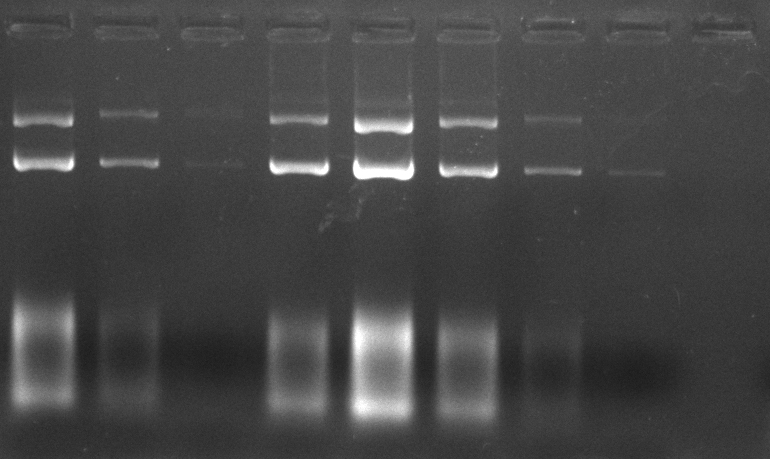
\includegraphics[width=7cm]{ima1}};
\begin{scope}[font=\scriptsize]
\node at (-3.15,2.3) {1};
\node at (-2.35,2.3) {2};
\node at (-1.55,2.3) {3};
\node at (-0.8,2.3) {4};
\node at (0,2.3) {5};
\node at (0.75,2.3) {6};
\node at (1.55,2.3) {7};
\node at (2.3,2.3) {8};
\node at (3.1,2.3) {9};
\draw (3.6,1.15) -- (3.75,1.15) -- (3.85,1.45) -- (4,1.45)  node[right] {gDNA};
\draw (3.6,1) -- (4,1) node[right] {pDNA (oc)};
\draw (3.6,0.55) -- (4,0.55) node[right] {pDNA (sc)};
\draw (3.6,-1) -- (4,-1) node[right] {RNA HMw};
\draw (3.6,-1.6) -- (4,-1.6) node[right] {RNA LMw};
\end{scope}
\end{tikzpicture}
\caption[Eletroforese em gel de agarose ao longo do processo de diafiltração]{Eletroforese em gel de agarose das amostras ao longo do processo de diafiltração: (1) Solução inicial (lisado); (2) permeado total recolhido; (3) concentrado após diafiltração; (4--8) amostras de permeado para VDF de 0.04, 0.15, 0.5, 1.5 e 2.5 respetivamente. (oc) indica a isoforma circular-aberta; (sc) indica a isoforma super-enrolada.}
\label{fig:2bart3}
\end{figure}
A técnica analítica de HIC utilizada para quantificar o DNA plasmídico (secção~\ref{subsubsec:2p3p1art3}) foi igualmente usada para obter informação sobre o conteúdo de contaminantes e consequentemente a sua remoção (ver capítulo~\ref{cha:pra}). De particular importância é a possibilidade de relacionar a permeação do RNA com a remoção dos contaminantes hidrofóbicos (ver apêndice~\ref{app:2}).
\index{contaminantes!hidrofóbicos}%
\index{contaminantes!RNA|see{RNA}}%
\index{contaminantes!DNA genómico|see{DNA genómico}}%
\index{contaminantes!proteínas|see{proteínas}}%
Como é possível ver na figura~\ref{fig:2aart3}, o rendimento de permeação dos contaminantes hidrofóbicos é por regra elevado na primeira operação de membranas, o que indica uma reduzida remoção do RNA presente. A análise por eletroforese, mostrada na figura~\ref{fig:2bart3}, confirma a ideia que o RNA permeia através da membrana juntamente com o pDNA. 

Proteínas e gDNA foram quantificados com os métodos descritos na secção~\ref{subsec:2p3art3}. Os dados para a remoção de gDNA e de proteína total, obtidos respetivamente por PCR em tempo real e pelo método do BCA, são indicados na tabela~\ref{tab:2art3}.
\index{PCR}%
\index{BCA}%
Observou-se baixa remoção de proteínas durante a diafiltração dos lisados (ver testes MF-A), em concordância com o baixo rendimento de contaminantes hidrofílicos verificado na análise de HIC. Os resultados mostram que existe uma tendência para o gDNA se re-dissolver, a partir do conteúdo sólido suspenso, tal como os valores negativos de remoção indicam.
\index{DNA genómico!redissolução}%
\index{tampão!diafiltração}%
Uma vez que é necessário que os sólidos suspensos contactem com o tampão de diafiltração durante o processo de filtração (para obter rendimentos de recuperação elevados de pDNA), durante a otimização de um sistema de filtração para aplicações em larga escala este resultado mostra que é necessário controlar as tensões de corte que atuam no material sólido para minimizar a degradação mecânica do gDNA precipitado e para evitar assim a sua re-solubilização.
\index{DNA genómico}%
\index{tensão de corte}%
É importante realçar que este aspeto não deve ser visto como uma desvantagem inerente aos processos de membranas quando comparados com a centrifugação. Na realidade são esperadas tensões de corte superiores, neste último processo, em centrífugas industriais \cite{prather,theo,chamsart,levy00}.
\index{centrifugação}%  
\begin{table}%
\centering
\caption[Proteína total e DNA genómico (gDNA) nos permeados após diafiltração]{Proteína total e DNA genómico (gDNA) nos permeados após diafiltração (microfiltração) com diferentes tampões e as suas remoções (\remocaoum) na operação de difiltração (testes MF-A, MF-B e MF-C). Valores iniciais medidos nos lisados: 200\,\micro g/mL de proteína total e 13.4\,\micro g de gDNA.}
\label{tab:2art3}
\begin{threeparttable}
\begin{tabular*}{14cm}{l @{\extracolsep{\fill}} llll}
\toprule
Ensaio & Proteína [\micro g/mL] &  \remocaoum\ (\porcento) & gDNA [\micro g/mL] & \remocaoum (\porcento) \\
\midrule
MF-A & 61 & 7.7 & 43.0 & -865 \\
MF-B & 71 & -6.3 & 18.1 & -306 \\
MF-C & 172\tnote{a}/45 & 14\tnote{a}/33 & 2.4\tnote{a}/5.5 &71\tnote{a}/-44 \\
\bottomrule
\end{tabular*}
\begin{tablenotes}
\item[a]Imediatamente após precipitação com CaCl$_2$.
\end{tablenotes} 
\end{threeparttable}
\end{table}

\subsubsection{Ensaios MF-B}
\label{subsubsec:3p1p3art3}
\index{microfiltração!MF-B}%
Para tentar evitar a excessiva re-solubilização do gDNA investigou-se a possibilidade de manter a força iónica aproximadamente constante durante o processo de diafiltração, usando \tce{CH3COOK} 1\,M em Tris/HCl 10\,mM a pH 8.00 (tampão ``B'', secção~\ref{subsec:2p2art3}).
\index{tampão!MF-B}%
Estes ensaios foram denominados ensaios MF-B. Teoricamente, não é previsível que as permeações de pDNA e RNA, ou mesmo as suas polarizações de concentração se alterem, tal como indicado na figura~\ref{fig:3acart3}.
\begin{figure}
	\centering
	%!TEX root=testfigum.tex
\begin{tikzpicture}

%\draw[help lines] (0cm,0cm) grid (14cm,7cm);
\node[right,font=\scriptsize] at (0cm,4.75cm) {MF-B};
\node[right,font=\scriptsize] at (7cm,4.75cm) {MF-B};
\node[right,font=\large] at (0cm,5.5cm) {a)};
\node[right,font=\large] at (7cm,5.5cm) {b)};

\begin{axis}[%
%width=\figurewidth,
%height=\figureheight,
width=5cm,
height=5cm,
scale only axis,
xmin=0,
xmax=3,
xlabel={VDF},
ymin=0,
ymax=1.1,
ylabel={\permobs},
at={(0cm,0cm)},
anchor=south west,
name=plot1,
legend style={at={(6cm,-1.5cm)},legend columns=2,anchor=center,font=\scriptsize,draw=black,fill=white,legend cell align=left}
]
\addplot [
color=black,
solid,
%forget plot
]
table[row sep=crcr]{
0 0.9864253394\\
0.6558345643 0.9841628959\\
1.369276219 0.9864253394\\
1.861152142 0.9864253394\\
2.144756278 0.9864253394\\
2.614475628 0.9864253394\\
3 0.9864253394\\
};
\addlegendentry{\pVAX};

\addplot [
color=black,
dashed,
%forget plot
]
table[row sep=crcr]{
0 0.9954751131\\
0.2304283604 0.9954751131\\
0.5228951256 0.9977375566\\
0.8153618907 1\\
1.183161004 1\\
1.568685377 1\\
1.905465288 1\\
2.353028065 1\\
2.694239291 1\\
3 1\\
};
\addlegendentry{RNA 23\,S};

\addplot [
color=black,
dash pattern=on 1pt off 3pt on 3pt off 3pt,
%forget plot
]
table[row sep=crcr]{
0 0.9954751131\\
0.1949778434 0.9977375566\\
0.4342688331 0.9977375566\\
0.7355982275 1\\
1.107828656 1\\
1.435745938 1\\
1.772525849 1\\
2.104874446 1\\
2.627769572 0.9977375566\\
2.871491876 1\\
3 0.9977375566\\
};
\addlegendentry{RNA 16\,S};

\addplot [
color=black,
dotted,
%forget plot
]
table[row sep=crcr]{
0 0.9932126697\\
0.2481536189 0.9954751131\\
0.4963072378 0.9977375566\\
0.8242245199 0.9954751131\\
1.307237814 0.9977375566\\
1.688330871 0.9977375566\\
2.082717873 0.9977375566\\
2.742983752 0.9954751131\\
3 0.9977375566\\
};
\addlegendentry{RNA 5\,S};
\end{axis}

\begin{axis}[%
%width=\figurewidth,
%height=\figureheight,
width=5cm,
height=5cm,
scale only axis,
xmin=0,
xmax=3,
xlabel={VDF},
ymin=0,
ymax=2,
ylabel={\concm/\concb},
at={(7cm,0cm)},
anchor=south west,
%legend style={at={(0.97,0.03)},anchor=south east,font=\scriptsize,draw=black,fill=white,legend cell align=left}
]
\addplot [
color=black,
solid
]
table[row sep=crcr]{
0 1.679671458\\
0.5672082718 1.675564682\\
1.564254062 1.679671458\\
1.989660266 1.679671458\\
2.570162482 1.679671458\\
3 1.679671458\\
};
%\addlegendentry{\pVAX};

\addplot [
color=black,
dashed
]
table[row sep=crcr]{
0 1.162217659\\
0.3545051699 1.170431211\\
0.8197932053 1.170431211\\
1.280649926 1.170431211\\
1.732644018 1.174537988\\
2.184638109 1.170431211\\
2.649926145 1.170431211\\
3 1.170431211\\
};
%\addlegendentry{RNA 23\,S};

\addplot [
color=black,
dash pattern=on 1pt off 3pt on 3pt off 3pt
]
table[row sep=crcr]{
0 1.133470226\\
0.2880354505 1.133470226\\
0.9704579025 1.133470226\\
1.550960118 1.133470226\\
2.016248154 1.133470226\\
2.592319055 1.133470226\\
3 1.137577002\\
};
%\addlegendentry{RNA 16\,S};

\addplot [
color=black,
dotted
]
table[row sep=crcr]{
0 1.075975359\\
0.4165435746 1.075975359\\
0.8995568685 1.075975359\\
1.382570162 1.071868583\\
1.856720827 1.075975359\\
2.251107829 1.075975359\\
2.579025111 1.075975359\\
3 1.075975359\\
};
%\addlegendentry{RNA 5\,S};

\end{axis}
\end{tikzpicture}%
	\caption[Previsão das permeações e da polarização de concentração (MF-B)]{Permeações observadas (a) e polarização de concentração (b), para as várias espécies, em função do fator de diluição volumétrico (VDF) para os ensaios MF-B.}
	\label{fig:3acart3}
\end{figure}

Os resultados experimentais, apresentados na figura~\ref{fig:3eart3}, confirmam que a permeação de pDNA e dos contaminantes permanece elevada, com um ligeiro aumento no rendimento de recuperação do DNA plasmídico, que se observou ser (92.4$\pm$0.4)\porcento\ nestas condições. A retenção do pDNA foi de (4.4$\pm$0.1)\porcento, sugerindo assim um decréscimo na adsorção, o que conduz a uma melhor aproximação entre os resultados experimentais e as previsões teóricas. Como é possível verificar na tabela~\ref{tab:2art3}, a remoção de proteínas permaneceu baixa, mas observou-se uma variação significativa no conteúdo de gDNA nos permeados, obtendo-se uma redução de cerca de 60\%.
\index{DNA genómico!rendimento de remoção (MF)}%
\index{proteínas!rendimento de remoção (MF)}%
Este resultado sugere que a re-dissolução de gDNA pode de facto ser reduzida aumentando a força iónica do tampão de diafiltração. É possível que este aumento da força iónica possa ter dado origem a menores valores de re-dissolução de outros contaminantes, o que pode ter conduzido a uma menor adsorção do plasmídeo na membrana. 
\begin{figure}
	\centering
	\setlength\figureheight{6cm} 
	\setlength\figurewidth{6cm}
	% This file was created by matlab2tikz v0.3.3.
% Copyright (c) 2008--2013, Nico Schlömer <nico.schloemer@gmail.com>
% All rights reserved.
% 
% The latest updates can be retrieved from
%   http://www.mathworks.com/matlabcentral/fileexchange/22022-matlab2tikz
% where you can also make suggestions and rate matlab2tikz.
% 
% 
% 
\begin{tikzpicture}
%\draw[help lines] (-2,-2) grid (10,10);
\node[right,font=\scriptsize] at (0,5.75) {MF-B}; 
\begin{axis}[%
width=\figurewidth,
height=\figureheight,
scale only axis,
xmin=0,
xmax=3.2,
xlabel={VDF},
ymin=0,
ymax=1.05,
ylabel={Rendimento de permeação},
legend style={at={(1.03,0.5)},anchor=west,font=\scriptsize,draw=black,fill=white,legend cell align=left}
]
\addplot [
color=black,
solid
]
table[row sep=crcr]{
0 -0.002155172414\\
0.08035714286 0.05603448276\\
0.2142857143 0.1530172414\\
0.375 0.2693965517\\
0.5669642857 0.3943965517\\
0.7544642857 0.5\\
0.9508928571 0.5862068966\\
1.174107143 0.6745689655\\
1.441964286 0.7521551724\\
1.866071429 0.8405172414\\
2.174107143 0.8857758621\\
2.549107143 0.9288793103\\
2.852678571 0.9504310345\\
3 0.9590517241\\
};
\addlegendentry{Permeação total};

\addplot [
color=black,
only marks,
mark=*,
mark options={solid,fill=white,draw=black}
]
table[row sep=crcr]{
0.04464 0.004310344828\\
0.04464 0.008620689655\\
0.1517857143 0.07327586207\\
0.1517857143 0.08836206897\\
0.5 0.3534482759\\
0.5 0.3642241379\\
1.5 0.7564655172\\
1.5 0.7737068966\\
2.5 0.8706896552\\
2.5 0.8836206897\\
3 0.9181034483\\
3 0.9245689655\\
};
\addlegendentry{\pVAX};

\addplot [
color=black,
only marks,
mark=triangle*,
mark options={solid,,rotate=180,fill=black,draw=black}
]
table[row sep=crcr]{
0.04464 0.002155172414\\
0.04464 0.01293103448\\
0.1517857143 0.09482758621\\
0.1517857143 0.07974137931\\
0.5 0.3534482759\\
0.5 0.3728448276\\
1.5 0.7543103448\\
1.5 0.7931034483\\
2.5 0.9288793103\\
2.5 0.8771551724\\
3 0.9418103448\\
3 0.9892241379\\
};
\addlegendentry{C. hidrofílicos};

\addplot [
color=black,
only marks,
mark=triangle*,
mark options={solid,fill=white,draw=black}
]
table[row sep=crcr]{
0.04464 0.002155172414\\
0.1517857143 0.06896551724\\
0.5 0.3362068966\\
0.5 0.3836206897\\
1.5 0.7392241379\\
1.5 0.8168103448\\
2.5 0.8577586207\\
2.5 0.974137931\\
3 0.9181034483\\
3 0.9181034483\\
};
\addlegendentry{C. hidrofóbicos};

\end{axis}
\end{tikzpicture}%
	\caption[Rendimentos de permeação de pDNA e contaminantes (MF-B)]{Rendimentos de permeação do pDNA, contaminantes hidrofílicos e contaminantes hidrofóbicos em função do fator de diluição volumétrico, para os ensaios MF-B.}
	\label{fig:3eart3}
\end{figure}

\subsubsection{Ensaios MF-C}
\label{subsubsec:3p1p4art3}
\index{microfiltração!MF-C}%
Estudou-se um novo aumento da força iónica da solução pela adição de 1\,M de \cacldois\ aos lisados, antes da diafiltração, e pelo uso do tampão ``C'' (ver secção~\ref{subsec:2p2art3}).
\index{tampão!MF-C}%
\index{cloreto de cálcio!microfiltração}%
A utilização do \cacldois\ teve também como finalidade precipitar o RNA presente. Estes ensaios são denominados ensaios MF-C. A adição de \cacldois\ aos lisados foi estudada previamente por Eon-Duval \et\ \cite{duvaltff,duval2} onde se demonstrou a eficácia deste sal na remoção de RNA por precipitação.
\index{cloreto de cálcio!precipitação de RNA}%
Pela aplicação do modelo, é esperado que a adição de 1\,M de \cacldois\ aos lisados não afete as permeações e polarização de concentração do plasmídeo e das várias espécies de RNA, tal como se pode verificar na figura~\ref{fig:3bdart3}. Só é esperado uma alteração para um poro com um raio inferior a 10\,nm, tal como se pode ver comparando a figura~\ref{fig:1art3}~(a) com a figura~\ref{fig:4abart3}~(a), e a figura~\ref{fig:1art3}~(b) com a figura~\ref{fig:4abart3}~(b), respetivamente. Os cromatogramas de HIC dos lisados, antes e depois da adição de \cacldois, mostrados na figura~\ref{fig:4cart3}, indicam que a concentração de pDNA não é afetada pela adição de \cacldois, ao mesmo tempo que mostram a elevada remoção dos contaminantes hidrofóbicos, tal como esperado.
\index{lisado!HIC}%
Durante o processo de diafiltração, a concentração destes compostos manteve-se muito reduzida, tal como se pode verificar a partir dos valores de remoção mostrados na figura~\ref{fig:3fart3}. Obteve-se um rendimento de remoção destes contaminantes de 91\% no final da diafiltração.
\index{contaminantes!rendimento de remoção}%
A análise por eletroforese, mostrada na figura~\ref{fig:4dart3}, confirma a elevada remoção do RNA conseguida com a adição de \cacldois, onde se pode constatar que praticamente todo o RNA de alto peso molecular (HMw\,RNA) e a maior parte do RNA de baixo peso molecular (LMw\,RNA), presente inicialmente nos lisados, é removido antes da diafiltração.
\index{AGE}%
Os contaminantes que não precipitam com a adição de \cacldois\ permeiam livremente pela membrana, tal como se pode verificar pelos valores de remoção obtidos exclusivamente para o passo de filtração, estando estes valores indicados na figura~\ref{fig:3fart3}, onde são denominados por ``apenas filtração''. Para além da elevada remoção de RNA obtida com a adição de \cacldois\ aos lisados, verificou-se também alguma precipitação de proteínas e especialmente gDNA (ver tabela~\ref{tab:2art3}). No entanto observou-se também uma maior adsorção de pDNA em comparação com os ensaios anteriores, cerca de 15\%, como indicam os valores de rendimento de permeação, (84$\pm$1)\%, e de retenção, (0.3$\pm$0.1)\%.\index{DNA plasmídico!adsorção}
\begin{figure}[!t]
	\centering
	%!TEX root=testfigum.tex
\begin{tikzpicture}

%\draw[help lines] (0cm,0cm) grid (14cm,7cm);
\node[right,font=\scriptsize] at (0cm,4.75cm) {MF-C};
\node[right,font=\scriptsize] at (7cm,4.75cm) {MF-C};
\node[right,font=\large] at (0,5.5) {a)};
\node[right,font=\large] at (7,5.5) {b)};

\begin{axis}[%
%width=\figurewidth,
%height=\figureheight,
width=5cm,
height=5cm,
scale only axis,
xmin=0,
xmax=3,
xlabel={VDF},
ymin=0,
ymax=1.1,
ylabel={\permobs},
at={(0cm,0cm)},
anchor=south west,
name=plot1,
legend style={at={(6cm,-1.5cm)},legend columns=2,anchor=center,font=\scriptsize,draw=black,fill=white,legend cell align=left}
]
\addplot [
color=black,
solid,
%forget plot
]
table[row sep=crcr]{
0 0.993227991 \\
1.544247788 0.993227991\\
2.654867257 0.993227991\\
3 0.993227991\\
};
\addlegendentry{\pVAX};

\addplot [
color=black,
dashed,
%forget plot
]
table[row sep=crcr]{
0.004424779 0.993227991\\
0.530973451 0.997742664\\
1.911504425 0.997742664\\
2.694690265 0.997742664\\
3 0.997742664\\
};
\addlegendentry{RNA 23\,S};

\addplot [
color=black,
dash pattern=on 1pt off 3pt on 3pt off 3pt,
%forget plot
]
table[row sep=crcr]{
0 0.995485327\\
0.654867257 0.995485327\\
1.628318584 0.993227991\\
2.305309735 0.995485327\\
2.787610619 0.995485327\\
3 0.995485327\\
};
\addlegendentry{RNA 16\,S};

\addplot [
color=black,
dotted,
%forget plot
]
table[row sep=crcr]{
0 0.995485327\\
0.867256637 0.995485327\\
2.110619469 0.997742664\\
2.738938053 0.995485327\\
2.995575221 0.995485327\\
};
\addlegendentry{RNA 5\,S};
\end{axis}

\begin{axis}[%
%width=\figurewidth,
%height=\figureheight,
width=5cm,
height=5cm,
scale only axis,
xmin=0,
xmax=3,
xlabel={VDF},
ymin=0,
ymax=2,
ylabel={\concm/\concb},
at={(7cm,0cm)},
anchor=south west,
%legend style={at={(0.97,0.03)},anchor=south east,font=\scriptsize,draw=black,fill=white,legend cell align=left}
]
\addplot [
color=black,
solid
]
table[row sep=crcr]{
0	1.503080082\\
1.728212703	1.503080082\\
3	1.503080082\\
};
%\addlegendentry{\pVAX};

\addplot [
color=black,
dashed
]
table[row sep=crcr]{
0	1.170431211
1.426883309	1.170431211\\
2.042836041	1.170431211\\
3	1.170431211\\
};
%\addlegendentry{RNA 23\,S};

\addplot [
color=black,
dash pattern=on 1pt off 3pt on 3pt off 3pt
]
table[row sep=crcr]{
0.00E+00	1.137577002\\
1.316100443	1.133470226\\
2.127031019	1.137577002\\
3	1.137577002\\
};
%\addlegendentry{RNA 16\,S};

\addplot [
color=black,
dotted
]
table[row sep=crcr]{
0.00E+00	1.071868583\\
0.740029542	1.071868583\\
1.612998523	1.071868583\\
2.246676514	1.071868583\\
3	1.075975359\\
};
%\addlegendentry{RNA 5\,S};

\end{axis}
\end{tikzpicture}%
	\caption[Previsão das permeações e da polarização de concentração (MF-C)]{Permeações observadas (a) e polarização de concentração (b), para as várias espécies, em função do fator de diluição volumétrico (VDF) para os ensaios MF-C.}
	\label{fig:3bdart3}
\end{figure}
\begin{figure}[!t]
	\centering
	%!TEX root=testfigum.tex
\begin{tikzpicture}

%\draw[help lines] (0cm,0cm) grid (14cm,7cm);
\node[right,font=\scriptsize] at (0cm,4.75cm) {CaCl$_2$\ 1\,M};
\node[left,font=\scriptsize] at (12cm,4.75cm) {CaCl$_2$\ 1\,M};
\node[right,font=\large] at (0,5.5) {a)};
\node[right,font=\large] at (7,5.5) {b)};

\begin{axis}[%
%width=\figurewidth,
%height=\figureheight,
width=5cm,
height=5cm,
scale only axis,
xmode=log,
xmin=1,
xmax=100,
xminorticks=true,
xlabel={\raioporo\,[nm]},
ymin=0,
ymax=1.1,
ylabel={\permobs},
at={(0cm,5cm)},
anchor=north west,
name=plot1,
legend style={at={(6cm,-1.5cm)},legend columns=2,anchor=center,font=\scriptsize,draw=black,fill=white,legend cell align=left}
]
\addplot [
color=black,
solid,
%forget plot
]
table[row sep=crcr]{
1 0.018480493\\
1.4 0.039014374\\
1.89 0.063655031\\
2.23 0.084188912\\
2.73 0.12936345\\
3.35 0.193018481\\
3.97 0.275154004\\
4.58 0.369609856\\
5.21 0.464065708\\
6.01 0.59137577\\
6.98 0.751540041\\
7.94 0.90349076\\
8.85 0.975359343\\
9.87 0.995893224\\
13.85 1\\
100 1\\
};
\addlegendentry{\pVAX};

\addplot [
color=black,
dashed,
%forget plot
]
table[row sep=crcr]{
1 0.232032854\\
1.15 0.316221766\\
1.38 0.41889117\\
1.77 0.626283368\\
2.07 0.76386037\\
2.62 0.90349076\\
3.19 0.969199179\\
4.08 0.997946612\\
5.58 1\\
100 1\\
};
\addlegendentry{RNA 23\,S};

\addplot [
color=black,
dash pattern=on 1pt off 3pt on 3pt off 3pt,
%forget plot
]
table[row sep=crcr]{
1 0.400410678\\
1.15 0.509240246\\
1.35 0.62422998\\
1.58 0.737166324\\
1.91 0.850102669\\
2.62 0.944558522\\
3.84 0.981519507\\
5.65 0.993839836\\
8.38 0.997946612\\
22.14 0.997946612\\
100 1\\
};
\addlegendentry{RNA 16\,S};

\addplot [
color=black,
dotted,
%forget plot
]
table[row sep=crcr]{
1 0.515400411\\
1.26 0.609856263\\
1.77 0.751540041\\
2.47 0.856262834\\
3.61 0.917864476\\
5.17 0.952772074\\
8.32 0.979466119\\
13.67 0.991786448\\
19.72 0.995893224\\
39.17 1\\
100 1\\
};
\addlegendentry{RNA 5\,S};
\end{axis}

\begin{axis}[%
%width=\figurewidth,
%height=\figureheight,
width=5cm,
height=5cm,
scale only axis,
xmode=log,
xmin=1,
xmax=100,
xlabel={\raioporo\,[nm]},
ymin=-10,
ymax=120,
ylabel={\concm/\concb},
at={(7cm,0cm)},
anchor=south west,
%legend style={at={(0.97,0.97)},anchor=north east,font=\scriptsize,draw=black,fill=white,legend cell align=left}
]
\addplot [
color=black,
solid
]
table[row sep=crcr]{
1 56.18069815\\
1.50675119 55.68788501\\
2.498193723 55.44147844\\
3.764156364 55.44147844\\
4.781071325 53.71663244\\
6.156267855 51.00616016\\
7.505349485 47.06365503\\
8.42977579 41.88911704\\
9.598333721 33.75770021\\
11.62202751 24.64065708\\
13.88139889 17.49486653\\
17.75244435 10.59548255\\
26.74851665 5.420944559\\
42.56769351 2.95687885\\
69.14529137 1.971252567\\
100 1.478439425\\
};
%\addlegendentry{\pVAX};

\addplot [
color=black,
dashed
]
table[row sep=crcr]{
1.261508577 120\\
1.496491257 114.3326489\\
1.703938854 108.4188912\\
1.874981697 102.9979466\\
2.063193967 95.35934292\\
2.239486083 86.98151951\\
2.549929597 71.70431211\\
2.786787524 62.83367556\\
3.066527645 53.96303901\\
3.713068298 37.94661191\\
4.227783696 30.06160164\\
5.154258219 20.94455852\\
6.457865875 13.30595483\\
9.664139821 6.652977413\\
15.6980496 3.449691992\\
24.30841695 1.971252567\\
41.13801413 1.232032854\\
79.27017044 0.985626283\\
100 1.232032854\\
};
%\addlegendentry{RNA 23\,S};

\addplot [
color=black,
dash pattern=on 1pt off 3pt on 3pt off 3pt
]
table[row sep=crcr]{
1.085446215 120.2464066\\
1.252918577 109.650924\\
1.407239291 101.5195072\\
1.613299999 89.19917864\\
1.751150378 81.31416838\\
1.874981697 74.16837782\\
2.105921297 61.60164271\\
2.447507524 48.04928131\\
2.943355571 34.25051335\\
3.868450927 20.69815195\\
4.684067506 14.78439425\\
6.820683433 7.392197125\\
10 4.188911704\\
14.66128739 2.710472279\\
21.79108888 1.724845996\\
33.28550827 1.232032854\\
78.19429601 0.985626283\\
100 1.232032854\\
};
%\addlegendentry{RNA 16\,S};

\addplot [
color=black,
dotted
]
table[row sep=crcr]{
1.027707288 0.492813142\\
1.763156251 0.739219713\\
3.216758058 0.985626283\\
5.789102992 0.985626283\\
10.92888027 0.985626283\\
17.87415497 0.985626283\\
25.1532132 0.985626283\\
41.7040317 0.985626283\\
67.742393 0.985626283\\
100 0.985626283\\
};
%\addlegendentry{RNA 5\,S};

\end{axis}
\end{tikzpicture}%
	\caption[Permeação e da polarização de concentração em função de \raioporo\ (MF-C)]{Previsão das permeações observadas (a) e da polarização de concentração (b) para o plasmídeo (usando o modelo CSC) e para as várias espécies de RNA (usando o modelo FJC), para as condições experimentais dos ensaios MF-C.}
	\label{fig:4abart3}
\end{figure}
\begin{figure}[!t]
	\centering
	\setlength\figureheight{6cm} 
	\setlength\figurewidth{6cm}
	% This file was created by matlab2tikz v0.3.3.
% Copyright (c) 2008--2013, Nico Schlömer <nico.schloemer@gmail.com>
% All rights reserved.
% 
% The latest updates can be retrieved from
%   http://www.mathworks.com/matlabcentral/fileexchange/22022-matlab2tikz
% where you can also make suggestions and rate matlab2tikz.
% 
% 
% 
\begin{tikzpicture}

%\draw[help lines] (-2,-1) grid (12,10);
\node[right,font=\scriptsize] at (0,5.75) {HIC};

\begin{axis}[%
width=\figurewidth,
height=\figureheight,
scale only axis,
xmin=0,
xmax=8,
xlabel={\volretencao\,[mL]},
ymin=-100,
ymax=1400,
ylabel={Absorvância 260\,nm\,[mAU]},
legend style={at={(1.03,0.5)},anchor=west,font=\scriptsize,draw=black,fill=white,legend cell align=left}
]
\addplot [
color=black,
solid
]
table[row sep=crcr]{
0 -0.019\\
0.01 -0.027\\
0.02 -0.035\\
0.0299 -0.036\\
0.0399 -0.03\\
0.0499 -0.033\\
0.0599 -0.037\\
0.0699 -0.036\\
0.0799 -0.035\\
0.0898 -0.027\\
0.0998 -0.014\\
0.1098 -0.007\\
0.1198 0\\
0.1298 0.004\\
0.1398 0.003\\
0.1497 0.01\\
0.1597 -0.001\\
0.1697 -0.004\\
0.1797 -0.009\\
0.1897 -0.016\\
0.1997 -0.011\\
0.2096 -0.009\\
0.2196 -0.008\\
0.2296 -0.003\\
0.2396 -0.005\\
0.2496 -0.001\\
0.2596 -0.002\\
0.2695 -0.004\\
0.2795 0.003\\
0.2895 0.007\\
0.2995 0.014\\
0.3095 0.018\\
0.3195 0.012\\
0.3294 0.001\\
0.3394 -0.008\\
0.3494 -0.015\\
0.3594 -0.013\\
0.3694 -0.005\\
0.3794 -0.009\\
0.3893 -0.012\\
0.3993 -0.015\\
0.4093 -0.018\\
0.4193 -0.015\\
0.4293 -0.009\\
0.4393 -0.001\\
0.4492 0.002\\
0.4592 0.002\\
0.4692 -0.005\\
0.4792 -0.009\\
0.4892 -0.013\\
0.4992 -0.011\\
0.5091 -0.007\\
0.5191 -0.009\\
0.5291 -0.005\\
0.5391 -0.001\\
0.5491 -0.006\\
0.5591 -0.007\\
0.569 -0.01\\
0.579 -0.012\\
0.589 -0.002\\
0.599 0.002\\
0.609 0.01\\
0.619 0.021\\
0.6289 0.19\\
0.6389 1.395\\
0.6489 6.534\\
0.6589 20.878\\
0.6689 49.858\\
0.6788 93.094\\
0.6888 141.194\\
0.6988 182.108\\
0.7088 206.022\\
0.7188 209.901\\
0.7288 198.133\\
0.7387 178.908\\
0.7487 159.052\\
0.7587 141.27\\
0.7687 125.977\\
0.7787 112.866\\
0.7887 101.507\\
0.7986 91.696\\
0.8086 82.938\\
0.8186 74.954\\
0.8286 67.661\\
0.8386 61.03\\
0.8486 54.997\\
0.8585 49.571\\
0.8685 44.715\\
0.8785 40.339\\
0.8885 36.396\\
0.8985 32.872\\
0.9085 29.73\\
0.9184 26.929\\
0.9284 24.477\\
0.9384 22.286\\
0.9484 20.32\\
0.9584 18.569\\
0.9684 17.008\\
0.9783 15.614\\
0.9883 14.391\\
0.9983 13.292\\
1.0083 12.302\\
1.0183 11.392\\
1.0283 10.573\\
1.0382 9.826\\
1.0482 9.145\\
1.0582 8.556\\
1.0682 8.023\\
1.0782 7.543\\
1.0882 7.129\\
1.0981 6.805\\
1.1081 6.65\\
1.1181 6.831\\
1.1281 7.776\\
1.1381 10.318\\
1.1481 15.964\\
1.158 26.751\\
1.168 43.73\\
1.178 65.65\\
1.188 90.042\\
1.198 115.814\\
1.208 143.843\\
1.2179 176.43\\
1.2279 215.003\\
1.2379 257.983\\
1.2479 300.647\\
1.2579 337.134\\
1.2679 364.247\\
1.2778 381.575\\
1.2878 390.139\\
1.2978 391.8\\
1.3078 388.54\\
1.3178 381.851\\
1.3277 372.628\\
1.3377 361.564\\
1.3477 349.15\\
1.3577 335.722\\
1.3677 321.637\\
1.3777 307.336\\
1.3876 293\\
1.3976 278.823\\
1.4076 264.965\\
1.4176 251.523\\
1.4276 238.515\\
1.4376 225.967\\
1.4475 214.022\\
1.4575 202.547\\
1.4675 191.575\\
1.4775 181.196\\
1.4875 171.418\\
1.4975 162.227\\
1.5074 153.667\\
1.5174 145.72\\
1.5274 138.329\\
1.5374 131.535\\
1.5474 125.387\\
1.5574 119.91\\
1.5673 115.161\\
1.5773 111.266\\
1.5873 108.282\\
1.5973 106.281\\
1.6073 105.356\\
1.6173 105.601\\
1.6272 107.076\\
1.6372 109.758\\
1.6472 113.688\\
1.6572 118.754\\
1.6672 124.737\\
1.6772 131.422\\
1.6871 138.575\\
1.6971 145.945\\
1.7071 153.198\\
1.7171 160.127\\
1.7271 166.544\\
1.7371 172.221\\
1.747 177.006\\
1.757 180.904\\
1.767 183.675\\
1.777 185.395\\
1.787 186.136\\
1.797 185.971\\
1.8069 185.004\\
1.8169 183.284\\
1.8269 180.932\\
1.8369 178.072\\
1.8469 174.758\\
1.8569 171.015\\
1.8668 167.191\\
1.8768 163.239\\
1.8868 159.093\\
1.8968 155.139\\
1.9068 151.314\\
1.9168 147.53\\
1.9267 144.013\\
1.9367 140.911\\
1.9467 138.162\\
1.9567 135.824\\
1.9667 134.278\\
1.9766 133.964\\
1.9866 135.041\\
1.9966 137.163\\
2.0066 139.688\\
2.0166 142.054\\
2.0266 143.534\\
2.0365 144.044\\
2.0465 143.93\\
2.0565 143.427\\
2.0665 142.655\\
2.0765 141.606\\
2.0865 140.351\\
2.0964 138.954\\
2.1064 137.489\\
2.1164 135.923\\
2.1264 134.345\\
2.1364 132.716\\
2.1464 131.055\\
2.1563 129.395\\
2.1663 127.614\\
2.1763 125.381\\
2.1863 122.603\\
2.1963 119.269\\
2.2063 115.504\\
2.2162 111.339\\
2.2262 107.073\\
2.2362 102.903\\
2.2462 98.825\\
2.2562 94.88\\
2.2662 91.154\\
2.2761 87.489\\
2.2861 84.053\\
2.2961 80.802\\
2.3061 77.721\\
2.3161 74.893\\
2.3261 72.308\\
2.336 69.821\\
2.346 67.468\\
2.356 65.325\\
2.366 63.372\\
2.376 61.526\\
2.386 59.845\\
2.3959 58.307\\
2.4059 56.909\\
2.4159 55.681\\
2.4259 54.601\\
2.4359 53.581\\
2.4459 52.606\\
2.4558 51.684\\
2.4658 50.803\\
2.4758 49.953\\
2.4858 49.17\\
2.4958 48.465\\
2.5058 47.849\\
2.5157 47.3\\
2.5257 46.723\\
2.5357 45.997\\
2.5457 45.092\\
2.5557 43.969\\
2.5657 42.704\\
2.5756 41.45\\
2.5856 40.263\\
2.5956 38.516\\
2.6056 37.265\\
2.6156 37.044\\
2.6255 36.901\\
2.6355 36.632\\
2.6455 36.091\\
2.6555 35.367\\
2.6655 34.631\\
2.6755 34.027\\
2.6854 33.598\\
2.6954 33.238\\
2.7054 32.899\\
2.7154 32.589\\
2.7254 32.3\\
2.7354 32.028\\
2.7453 31.766\\
2.7553 31.511\\
2.7653 31.266\\
2.7753 31.028\\
2.7853 30.799\\
2.7953 30.589\\
2.8052 30.39\\
2.8152 30.193\\
2.8252 30.004\\
2.8352 29.816\\
2.8452 29.626\\
2.8552 29.452\\
2.8651 29.293\\
2.8751 29.143\\
2.8851 28.994\\
2.8951 28.84\\
2.9051 28.687\\
2.9151 28.53\\
2.925 28.383\\
2.935 28.251\\
2.945 28.132\\
2.955 28.017\\
2.965 27.899\\
2.975 27.779\\
2.9849 27.655\\
2.9949 27.537\\
3.0049 27.43\\
3.0149 27.335\\
3.0249 27.237\\
3.0349 27.127\\
3.0448 27.017\\
3.0548 26.917\\
3.0648 26.839\\
3.0748 26.768\\
3.0848 26.694\\
3.0948 26.617\\
3.1047 26.522\\
3.1147 26.426\\
3.1247 26.347\\
3.1347 26.275\\
3.1447 26.206\\
3.1547 26.135\\
3.1646 26.055\\
3.1746 25.973\\
3.1846 25.895\\
3.1946 25.836\\
3.2046 25.796\\
3.2146 25.755\\
3.2245 25.71\\
3.2345 25.654\\
3.2445 25.576\\
3.2545 25.482\\
3.2645 25.383\\
3.2745 25.295\\
3.2844 25.216\\
3.2944 25.139\\
3.3044 25.071\\
3.3144 24.988\\
3.3244 24.9\\
3.3343 24.828\\
3.3443 24.76\\
3.3543 24.709\\
3.3643 24.656\\
3.3743 24.592\\
3.3843 24.524\\
3.3942 24.448\\
3.4042 24.383\\
3.4142 24.332\\
3.4242 24.283\\
3.4342 24.225\\
3.4442 24.163\\
3.4541 24.101\\
3.4641 24.028\\
3.4741 23.958\\
3.4841 23.9\\
3.4941 23.838\\
3.5041 23.777\\
3.514 23.709\\
3.524 23.632\\
3.534 23.554\\
3.544 23.479\\
3.554 23.425\\
3.564 23.386\\
3.5739 23.34\\
3.5839 23.284\\
3.5939 23.214\\
3.6039 23.129\\
3.6139 23.05\\
3.6239 22.98\\
3.6338 22.924\\
3.6438 22.87\\
3.6538 22.816\\
3.6638 22.758\\
3.6738 22.69\\
3.6838 22.622\\
3.6937 22.563\\
3.7037 22.508\\
3.7137 22.452\\
3.7237 22.395\\
3.7337 22.33\\
3.7437 22.259\\
3.7536 22.194\\
3.7636 22.132\\
3.7736 22.076\\
3.7836 22.027\\
3.7936 21.974\\
3.8036 21.911\\
3.8135 21.846\\
3.8235 21.778\\
3.8335 21.718\\
3.8435 21.672\\
3.8535 21.632\\
3.8635 21.592\\
3.8734 21.549\\
3.8834 21.497\\
3.8934 21.447\\
3.9034 21.411\\
3.9134 21.386\\
3.9234 21.36\\
3.9333 21.328\\
3.9433 21.282\\
3.9533 21.215\\
3.9633 21.149\\
3.9733 21.087\\
3.9832 21.046\\
3.9932 21.031\\
4.0032 21.034\\
4.0132 21.059\\
4.0232 21.104\\
4.0332 21.184\\
4.0431 21.319\\
4.0531 21.522\\
4.0631 21.791\\
4.0731 22.114\\
4.0831 22.478\\
4.0931 22.874\\
4.103 23.313\\
4.113 23.811\\
4.123 24.38\\
4.133 25.022\\
4.143 25.708\\
4.153 26.441\\
4.1629 27.195\\
4.1729 27.981\\
4.1829 28.819\\
4.1929 29.714\\
4.2029 30.673\\
4.2129 31.683\\
4.2228 32.725\\
4.2328 33.784\\
4.2428 34.869\\
4.2528 36.015\\
4.2628 37.226\\
4.2728 38.502\\
4.2827 39.833\\
4.2927 41.197\\
4.3027 42.583\\
4.3127 43.995\\
4.3227 45.48\\
4.3327 47.062\\
4.3426 48.726\\
4.3526 50.467\\
4.3626 52.277\\
4.3726 54.137\\
4.3826 56.057\\
4.3926 58.097\\
4.4025 60.273\\
4.4125 62.566\\
4.4225 64.981\\
4.4325 67.499\\
4.4425 70.082\\
4.4525 72.779\\
4.4624 75.607\\
4.4724 78.6\\
4.4824 81.758\\
4.4924 85.067\\
4.5024 88.524\\
4.5124 92.168\\
4.5223 96.001\\
4.5323 99.838\\
4.5423 104.002\\
4.5523 108.416\\
4.5623 113.111\\
4.5723 117.794\\
4.5822 122.81\\
4.5922 128.01\\
4.6022 133.431\\
4.6122 139.181\\
4.6222 145.331\\
4.6321 151.463\\
4.6421 158.168\\
4.6521 165.342\\
4.6621 172.564\\
4.6721 180.001\\
4.6821 188.174\\
4.692 196.972\\
4.702 205.881\\
4.712 215.77\\
4.722 226.435\\
4.732 237.199\\
4.742 249.224\\
4.7519 261.725\\
4.7619 274.933\\
4.7719 289.045\\
4.7819 304.941\\
4.7919 321.354\\
4.8019 338.586\\
4.8118 356.464\\
4.8218 376.298\\
4.8318 396.392\\
4.8418 419.052\\
4.8518 442.328\\
4.8618 466.51\\
4.8717 491.102\\
4.8817 517.812\\
4.8917 544.121\\
4.9017 573.124\\
4.9117 602.431\\
4.9217 632.372\\
4.9316 662.205\\
4.9416 693.922\\
4.9516 724.759\\
4.9616 755.598\\
4.9716 786.274\\
4.9816 818.718\\
4.9915 849.367\\
5.0015 881.212\\
5.0115 911.081\\
5.0215 939.511\\
5.0315 966.774\\
5.0415 994.583\\
5.0514 1020.398\\
5.0614 1044.703\\
5.0714 1066.612\\
5.0814 1087.571\\
5.0914 1105.213\\
5.1014 1122.165\\
5.1113 1136.911\\
5.1213 1149.573\\
5.1313 1159.813\\
5.1413 1168.177\\
5.1513 1173.283\\
5.1613 1176.21\\
5.1712 1177.179\\
5.1812 1176.304\\
5.1912 1173.521\\
5.2012 1168.471\\
5.2112 1161.162\\
5.2212 1151.598\\
5.2311 1140.219\\
5.2411 1127.596\\
5.2511 1113.821\\
5.2611 1098.699\\
5.2711 1082.26\\
5.281 1064.521\\
5.291 1045.222\\
5.301 1025.101\\
5.311 1004.692\\
5.321 983.791\\
5.331 962.31\\
5.3409 940.38\\
5.3509 917.796\\
5.3609 894.563\\
5.3709 871.307\\
5.3809 848.353\\
5.3909 825.488\\
5.4008 802.664\\
5.4108 780.055\\
5.4208 756.957\\
5.4308 733.805\\
5.4408 711.081\\
5.4508 688.889\\
5.4607 667.142\\
5.4707 645.836\\
5.4807 624.886\\
5.4907 603.815\\
5.5007 582.913\\
5.5107 562.613\\
5.5206 542.964\\
5.5306 523.813\\
5.5406 505.411\\
5.5506 487.065\\
5.5606 468.759\\
5.5706 450.788\\
5.5805 433.381\\
5.5905 416.573\\
5.6005 400.371\\
5.6105 384.796\\
5.6205 369.309\\
5.6305 353.947\\
5.6404 338.91\\
5.6504 324.382\\
5.6604 310.446\\
5.6704 297.185\\
5.6804 284.282\\
5.6904 271.606\\
5.7003 259.143\\
5.7103 247.032\\
5.7203 235.355\\
5.7303 224.232\\
5.7403 213.695\\
5.7503 203.486\\
5.7602 193.528\\
5.7702 183.824\\
5.7802 174.412\\
5.7902 165.429\\
5.8002 157.029\\
5.8102 148.999\\
5.8201 141.333\\
5.8301 133.898\\
5.8401 126.664\\
5.8501 119.698\\
5.8601 113.077\\
5.8701 106.939\\
5.88 101.12\\
5.89 95.41\\
5.9 90.277\\
5.91 85.153\\
5.92 80.064\\
5.9299 75.595\\
5.9399 71.275\\
5.9499 67.086\\
5.9599 63.377\\
5.9699 59.731\\
5.9799 56.107\\
5.9898 52.783\\
5.9998 49.76\\
6.0098 46.878\\
6.0198 44.096\\
6.0298 41.642\\
6.0398 39.256\\
6.0497 36.895\\
6.0597 34.813\\
6.0697 32.787\\
6.0797 30.854\\
6.0897 29.181\\
6.0997 27.523\\
6.1096 26.005\\
6.1196 24.561\\
6.1296 23.171\\
6.1396 21.87\\
6.1496 20.675\\
6.1596 19.579\\
6.1695 18.561\\
6.1795 17.604\\
6.1895 16.71\\
6.1995 15.852\\
6.2095 15.044\\
6.2195 14.299\\
6.2294 13.615\\
6.2394 12.978\\
6.2494 12.377\\
6.2594 11.803\\
6.2694 11.238\\
6.2794 10.708\\
6.2893 10.24\\
6.2993 9.818\\
6.3093 9.432\\
6.3193 9.072\\
6.3293 8.696\\
6.3393 8.31\\
6.3492 7.945\\
6.3592 7.616\\
6.3692 7.32\\
6.3792 7.066\\
6.3892 6.817\\
6.3992 6.556\\
6.4091 6.291\\
6.4191 6.041\\
6.4291 5.807\\
6.4391 5.592\\
6.4491 5.406\\
6.4591 5.231\\
6.469 5.056\\
6.479 4.883\\
6.489 4.709\\
6.499 4.539\\
6.509 4.386\\
6.519 4.253\\
6.5289 4.13\\
6.5389 3.998\\
6.5489 3.857\\
6.5589 3.712\\
6.5689 3.587\\
6.5788 3.462\\
6.5888 3.374\\
6.5988 3.28\\
6.6088 3.177\\
6.6188 3.074\\
6.6288 2.951\\
6.6387 2.845\\
6.6487 2.758\\
6.6587 2.68\\
6.6687 2.613\\
6.6787 2.537\\
6.6887 2.447\\
6.6986 2.346\\
6.7086 2.249\\
6.7186 2.177\\
6.7286 2.106\\
6.7386 2.034\\
6.7486 1.966\\
6.7585 1.875\\
6.7685 1.779\\
6.7785 1.695\\
6.7885 1.623\\
6.7985 1.554\\
6.8085 1.496\\
6.8184 1.442\\
6.8284 1.378\\
6.8384 1.3\\
6.8484 1.239\\
6.8584 1.187\\
6.8684 1.137\\
6.8783 1.085\\
6.8883 1.03\\
6.8983 0.95\\
6.9083 0.873\\
6.9183 0.806\\
6.9283 0.751\\
6.9382 0.705\\
6.9482 0.661\\
6.9582 0.604\\
6.9682 0.545\\
6.9782 0.491\\
6.9882 0.447\\
6.9981 0.418\\
7.0081 0.386\\
7.0181 0.348\\
7.0281 0.291\\
7.0381 0.232\\
7.0481 0.178\\
7.058 0.128\\
7.068 0.085\\
7.078 0.05\\
7.088 0.006\\
7.098 -0.036\\
7.108 -0.076\\
7.1179 -0.127\\
7.1279 -0.168\\
7.1379 -0.205\\
7.1479 -0.24\\
7.1579 -0.273\\
7.1679 -0.31\\
7.1778 -0.344\\
7.1878 -0.392\\
7.1978 -0.442\\
7.2078 -0.487\\
7.2178 -0.54\\
7.2277 -0.576\\
7.2377 -0.606\\
7.2477 -0.644\\
7.2577 -0.691\\
7.2677 -0.741\\
7.2777 -0.787\\
7.2876 -0.832\\
7.2976 -0.872\\
7.3076 -0.908\\
7.3176 -0.953\\
7.3276 -1.001\\
7.3376 -1.048\\
7.3475 -1.092\\
7.3575 -1.125\\
7.3675 -1.16\\
7.3775 -1.198\\
7.3875 -1.239\\
7.3975 -1.289\\
7.4074 -1.336\\
7.4174 -1.372\\
7.4274 -1.413\\
7.4374 -1.44\\
7.4474 -1.463\\
7.4574 -1.495\\
7.4673 -1.53\\
7.4773 -1.565\\
7.4873 -1.593\\
7.4973 -1.63\\
7.5073 -1.66\\
7.5173 -1.689\\
7.5272 -1.72\\
7.5372 -1.753\\
7.5472 -1.78\\
7.5572 -1.808\\
7.5672 -1.842\\
7.5772 -1.868\\
7.5871 -1.893\\
7.5971 -1.917\\
7.6071 -1.946\\
7.6171 -1.974\\
7.6271 -2.002\\
7.6371 -2.027\\
7.647 -2.046\\
7.657 -2.063\\
7.667 -2.084\\
7.677 -2.113\\
7.687 -2.157\\
7.697 -2.194\\
7.7069 -2.226\\
7.7169 -2.252\\
7.7269 -2.269\\
7.7369 -2.297\\
7.7469 -2.331\\
7.7569 -2.361\\
7.7668 -2.392\\
7.7768 -2.421\\
7.7868 -2.45\\
7.7968 -2.479\\
7.8068 -2.507\\
7.8168 -2.546\\
7.8267 -2.587\\
7.8367 -2.628\\
7.8467 -2.666\\
7.8567 -2.693\\
7.8667 -2.714\\
7.8766 -2.736\\
7.8866 -2.769\\
7.8966 -2.808\\
7.9066 -2.835\\
7.9166 -2.855\\
7.9266 -2.867\\
7.9365 -2.884\\
7.9465 -2.924\\
7.9565 -2.974\\
7.9665 -3.022\\
7.9765 -3.058\\
7.9865 -3.086\\
7.9964 -3.106\\
8.0064 -3.128\\
};
\addlegendentry{Lisado};

\addplot [
color=black,
dashed
]
table[row sep=crcr]{
0 0.004\\
0.01 0.013\\
0.02 0.03\\
0.03 0.033\\
0.04 0.029\\
0.05 0.031\\
0.06 0.02\\
0.07 0.016\\
0.08 0.016\\
0.09 0.008\\
0.1 0.005\\
0.11 0.002\\
0.12 0.011\\
0.13 0.024\\
0.14 0.025\\
0.15 0.077\\
0.16 0.076\\
0.17 0.081\\
0.18 0.081\\
0.19 0.05\\
0.2 0.026\\
0.21 0.012\\
0.22 0.008\\
0.23 0.003\\
0.24 0.018\\
0.25 0.024\\
0.26 0.025\\
0.2699 0.027\\
0.2799 0.012\\
0.2899 0\\
0.2999 0.001\\
0.3099 0.011\\
0.3199 0.019\\
0.3299 0.021\\
0.3399 0.018\\
0.3499 0.02\\
0.3599 0.024\\
0.3699 0.034\\
0.3799 0.043\\
0.3899 0.048\\
0.3999 0.042\\
0.4099 0.037\\
0.4199 0.035\\
0.4299 0.029\\
0.4399 0.029\\
0.4499 0.022\\
0.4599 0.022\\
0.4699 0.017\\
0.4799 0.016\\
0.4899 0.02\\
0.4999 0.03\\
0.5099 0.034\\
0.5199 0.028\\
0.5299 0.025\\
0.5399 0.022\\
0.5499 0.021\\
0.5599 0.012\\
0.5699 0.013\\
0.5799 0.007\\
0.5899 -0.006\\
0.5999 -0.012\\
0.6099 -0.01\\
0.6199 0\\
0.6299 0.231\\
0.6399 1.881\\
0.6499 8.558\\
0.6599 26.421\\
0.6699 60.45\\
0.6799 109.168\\
0.6899 161.548\\
0.6999 201.933\\
0.7099 220.925\\
0.7199 217.421\\
0.7299 198.659\\
0.7399 174.623\\
0.7499 152.487\\
0.7599 133.788\\
0.7699 118.052\\
0.7799 104.567\\
0.7899 92.763\\
0.7998 82.341\\
0.8098 73.246\\
0.8198 65.169\\
0.8298 57.978\\
0.8398 51.566\\
0.8498 45.872\\
0.8598 40.834\\
0.8698 36.402\\
0.8798 32.574\\
0.8898 29.183\\
0.8998 26.214\\
0.9098 23.616\\
0.9198 21.34\\
0.9298 19.358\\
0.9398 17.644\\
0.9498 16.125\\
0.9598 14.785\\
0.9698 13.596\\
0.9798 12.528\\
0.9898 11.575\\
0.9998 10.716\\
1.0098 9.956\\
1.0198 9.265\\
1.0298 8.633\\
1.0398 8.056\\
1.0498 7.528\\
1.0598 7.052\\
1.0698 6.619\\
1.0798 6.237\\
1.0898 5.9\\
1.0998 5.616\\
1.1098 5.444\\
1.1198 5.435\\
1.1298 5.757\\
1.1398 6.78\\
1.1498 9.359\\
1.1598 15.6\\
1.1698 27.502\\
1.1798 47.94\\
1.1898 76.56\\
1.1998 107.048\\
1.2098 139.75\\
1.2198 175.514\\
1.2298 213.632\\
1.2398 259.722\\
1.2498 312.451\\
1.2598 362.027\\
1.2698 400.841\\
1.2798 427.205\\
1.2898 440.221\\
1.2998 440.866\\
1.3098 431.909\\
1.3198 415.181\\
1.3297 394.793\\
1.3397 370.899\\
1.3497 345.58\\
1.3597 322.716\\
1.3697 300.86\\
1.3797 280.457\\
1.3897 263.035\\
1.3997 247.486\\
1.4097 233.293\\
1.4197 220.215\\
1.4297 208.013\\
1.4397 196.474\\
1.4497 185.499\\
1.4597 175.191\\
1.4697 165.291\\
1.4797 155.846\\
1.4897 146.933\\
1.4997 138.551\\
1.5097 130.691\\
1.5197 123.444\\
1.5297 116.771\\
1.5397 110.652\\
1.5497 105.137\\
1.5597 100.287\\
1.5697 96.177\\
1.5797 92.866\\
1.5897 90.521\\
1.5997 89.191\\
1.6097 88.933\\
1.6197 89.785\\
1.6297 91.778\\
1.6397 94.9\\
1.6497 99.017\\
1.6597 104.092\\
1.6697 109.909\\
1.6797 116.181\\
1.6897 122.693\\
1.6997 129.218\\
1.7097 135.513\\
1.7197 141.275\\
1.7297 146.458\\
1.7397 150.906\\
1.7497 154.52\\
1.7597 157.253\\
1.7697 159.09\\
1.7797 160.039\\
1.7897 160.108\\
1.7997 159.416\\
1.8097 158.065\\
1.8197 156.123\\
1.8297 153.694\\
1.8397 150.86\\
1.8497 147.727\\
1.8596 144.333\\
1.8696 140.745\\
1.8796 137.073\\
1.8896 133.373\\
1.8996 129.697\\
1.9096 126.134\\
1.9196 122.67\\
1.9296 119.335\\
1.9396 116.165\\
1.9496 113.181\\
1.9596 110.399\\
1.9696 107.819\\
1.9796 105.493\\
1.9896 103.356\\
1.9996 101.455\\
2.0096 99.823\\
2.0196 98.567\\
2.0296 97.738\\
2.0396 97.272\\
2.0496 97.049\\
2.0596 96.904\\
2.0696 96.703\\
2.0796 96.421\\
2.0896 96.108\\
2.0996 95.799\\
2.1096 95.563\\
2.1196 95.558\\
2.1296 95.999\\
2.1396 97.225\\
2.1496 99.482\\
2.1596 102.145\\
2.1696 104.214\\
2.1796 104.885\\
2.1896 103.7\\
2.1996 100.959\\
2.2096 97.501\\
2.2196 93.797\\
2.2296 90.042\\
2.2396 86.428\\
2.2496 83.006\\
2.2596 79.854\\
2.2696 76.996\\
2.2796 74.395\\
2.2896 71.995\\
2.2996 69.781\\
2.3096 67.703\\
2.3196 65.757\\
2.3296 63.952\\
2.3396 62.246\\
2.3496 60.602\\
2.3596 58.94\\
2.3696 57.191\\
2.3796 55.297\\
2.3895 53.265\\
2.3995 51.179\\
2.4095 49.13\\
2.4195 47.177\\
2.4295 45.411\\
2.4395 43.854\\
2.4495 42.491\\
2.4595 41.292\\
2.4695 40.225\\
2.4795 39.21\\
2.4895 38.146\\
2.4995 36.987\\
2.5095 35.722\\
2.5195 34.4\\
2.5295 33.109\\
2.5395 31.917\\
2.5495 30.838\\
2.5595 29.889\\
2.5695 29.072\\
2.5795 28.331\\
2.5895 27.758\\
2.5995 27.287\\
2.6095 26.916\\
2.6195 26.712\\
2.6295 26.461\\
2.6395 26.163\\
2.6495 25.708\\
2.6595 25.248\\
2.6695 24.849\\
2.6795 24.529\\
2.6895 24.272\\
2.6995 24.036\\
2.7095 23.809\\
2.7195 23.596\\
2.7295 23.389\\
2.7395 23.199\\
2.7495 23.03\\
2.7595 22.845\\
2.7695 22.663\\
2.7795 22.485\\
2.7895 22.309\\
2.7995 22.137\\
2.8095 21.984\\
2.8195 21.847\\
2.8295 21.701\\
2.8395 21.569\\
2.8495 21.449\\
2.8595 21.295\\
2.8695 21.158\\
2.8795 21.036\\
2.8895 20.914\\
2.8995 20.81\\
2.9095 20.701\\
2.9194 20.592\\
2.9294 20.465\\
2.9394 20.36\\
2.9494 20.269\\
2.9594 20.177\\
2.9694 20.09\\
2.9794 20.009\\
2.9894 19.914\\
2.9994 19.826\\
3.0094 19.736\\
3.0194 19.647\\
3.0294 19.567\\
3.0394 19.488\\
3.0494 19.415\\
3.0594 19.342\\
3.0694 19.258\\
3.0794 19.173\\
3.0894 19.1\\
3.0994 19.038\\
3.1094 18.967\\
3.1194 18.912\\
3.1294 18.84\\
3.1394 18.762\\
3.1494 18.699\\
3.1594 18.632\\
3.1694 18.577\\
3.1794 18.53\\
3.1894 18.477\\
3.1994 18.423\\
3.2094 18.369\\
3.2194 18.321\\
3.2294 18.263\\
3.2394 18.214\\
3.2494 18.166\\
3.2594 18.105\\
3.2694 18.044\\
3.2794 17.982\\
3.2894 17.923\\
3.2994 17.879\\
3.3094 17.839\\
3.3194 17.792\\
3.3294 17.735\\
3.3394 17.674\\
3.3494 17.616\\
3.3594 17.566\\
3.3694 17.53\\
3.3794 17.498\\
3.3894 17.453\\
3.3994 17.408\\
3.4094 17.351\\
3.4194 17.299\\
3.4294 17.27\\
3.4394 17.227\\
3.4493 17.193\\
3.4593 17.144\\
3.4693 17.082\\
3.4793 17.038\\
3.4893 16.999\\
3.4993 16.973\\
3.5093 16.952\\
3.5193 16.924\\
3.5293 16.883\\
3.5393 16.843\\
3.5493 16.802\\
3.5593 16.759\\
3.5693 16.705\\
3.5793 16.668\\
3.5893 16.625\\
3.5993 16.586\\
3.6093 16.552\\
3.6193 16.52\\
3.6293 16.482\\
3.6393 16.454\\
3.6493 16.416\\
3.6593 16.374\\
3.6693 16.337\\
3.6793 16.294\\
3.6893 16.261\\
3.6993 16.227\\
3.7093 16.196\\
3.7193 16.156\\
3.7293 16.118\\
3.7393 16.081\\
3.7493 16.039\\
3.7593 16.006\\
3.7693 15.971\\
3.7793 15.942\\
3.7893 15.928\\
3.7993 15.907\\
3.8093 15.885\\
3.8193 15.862\\
3.8293 15.829\\
3.8393 15.786\\
3.8493 15.76\\
3.8593 15.732\\
3.8693 15.7\\
3.8793 15.678\\
3.8893 15.646\\
3.8993 15.603\\
3.9093 15.54\\
3.9193 15.467\\
3.9293 15.384\\
3.9393 15.291\\
3.9493 15.212\\
3.9593 15.109\\
3.9693 14.977\\
3.9792 14.808\\
3.9892 14.631\\
3.9992 14.473\\
4.0092 14.35\\
4.0192 14.274\\
4.0292 14.239\\
4.0392 14.22\\
4.0492 14.205\\
4.0592 14.203\\
4.0692 14.26\\
4.0792 14.38\\
4.0892 14.574\\
4.0992 14.827\\
4.1092 15.079\\
4.1192 15.313\\
4.1292 15.564\\
4.1392 15.877\\
4.1492 16.24\\
4.1592 16.685\\
4.1692 17.172\\
4.1792 17.648\\
4.1892 18.088\\
4.1992 18.562\\
4.2092 19.036\\
4.2192 19.61\\
4.2292 20.225\\
4.2392 20.875\\
4.2492 21.496\\
4.2592 22.129\\
4.2692 22.739\\
4.2792 23.373\\
4.2892 24.05\\
4.2992 24.809\\
4.3092 25.557\\
4.3192 26.334\\
4.3292 27.063\\
4.3392 27.763\\
4.3492 28.459\\
4.3592 29.291\\
4.3692 30.145\\
4.3792 31.024\\
4.3892 31.909\\
4.3992 32.762\\
4.4092 33.567\\
4.4192 34.472\\
4.4292 35.417\\
4.4392 36.404\\
4.4492 37.394\\
4.4592 38.443\\
4.4692 39.398\\
4.4792 40.395\\
4.4892 41.403\\
4.4992 42.45\\
4.5091 43.51\\
4.5191 44.647\\
4.5291 45.73\\
4.5391 46.761\\
4.5491 47.735\\
4.5591 48.788\\
4.5691 49.821\\
4.5791 50.931\\
4.5891 52.013\\
4.5991 53.037\\
4.6091 53.948\\
4.6191 54.847\\
4.6291 55.705\\
4.6391 56.55\\
4.6491 57.352\\
4.6591 58.168\\
4.6691 58.849\\
4.6791 59.459\\
4.6891 59.963\\
4.6991 60.417\\
4.7091 60.823\\
4.7191 61.196\\
4.7291 61.499\\
4.7391 61.698\\
4.7491 61.779\\
4.7591 61.773\\
4.7691 61.724\\
4.7791 61.669\\
4.7891 61.578\\
4.7991 61.448\\
4.8091 61.213\\
4.8191 60.888\\
4.8291 60.489\\
4.8391 60.099\\
4.8491 59.76\\
4.8591 59.443\\
4.8691 59.096\\
4.8791 58.7\\
4.8891 58.226\\
4.8991 57.715\\
4.9091 57.248\\
4.9191 56.833\\
4.9291 56.44\\
4.9391 56.029\\
4.9491 55.553\\
4.9591 55.008\\
4.9691 54.43\\
4.9791 53.872\\
4.9891 53.366\\
4.9991 52.866\\
5.0091 52.341\\
5.0191 51.739\\
5.0291 51.061\\
5.039 50.34\\
5.049 49.619\\
5.059 48.951\\
5.069 48.288\\
5.079 47.602\\
5.089 46.869\\
5.099 46.066\\
5.109 45.241\\
5.119 44.459\\
5.129 43.722\\
5.139 43.03\\
5.149 42.332\\
5.159 41.595\\
5.169 40.826\\
5.179 40.041\\
5.189 39.303\\
5.199 38.641\\
5.209 37.995\\
5.219 37.362\\
5.229 36.715\\
5.239 36.013\\
5.249 35.321\\
5.259 34.622\\
5.269 33.965\\
5.279 33.33\\
5.289 32.691\\
5.299 32.007\\
5.309 31.227\\
5.319 30.45\\
5.329 29.637\\
5.339 28.817\\
5.349 28.052\\
5.359 27.247\\
5.369 26.363\\
5.379 25.475\\
5.389 24.527\\
5.399 23.562\\
5.409 22.676\\
5.419 21.778\\
5.429 20.854\\
5.439 19.914\\
5.449 18.979\\
5.459 17.992\\
5.469 17.008\\
5.479 16.132\\
5.489 15.273\\
5.499 14.426\\
5.509 13.616\\
5.519 12.768\\
5.529 11.886\\
5.539 11.076\\
5.549 10.339\\
5.559 9.652\\
5.5689 9.01\\
5.5789 8.371\\
5.5889 7.719\\
5.5989 7.07\\
5.6089 6.47\\
5.6189 5.929\\
5.6289 5.44\\
5.6389 4.993\\
5.6489 4.526\\
5.6589 4.048\\
5.6689 3.578\\
5.6789 3.15\\
5.6889 2.796\\
5.6989 2.503\\
5.7089 2.229\\
5.7189 1.938\\
5.7289 1.627\\
5.7389 1.301\\
5.7489 0.998\\
5.7589 0.758\\
5.7689 0.568\\
5.7789 0.416\\
5.7889 0.257\\
5.7989 0.07\\
5.8089 -0.145\\
5.8189 -0.343\\
5.8289 -0.499\\
5.8389 -0.607\\
5.8489 -0.683\\
5.8589 -0.77\\
5.8689 -0.894\\
5.8789 -1.028\\
5.8889 -1.155\\
5.8989 -1.257\\
5.9089 -1.326\\
5.9189 -1.385\\
5.9289 -1.459\\
5.9389 -1.547\\
5.9489 -1.655\\
5.9589 -1.741\\
5.9689 -1.807\\
5.9789 -1.852\\
5.9889 -1.881\\
5.9989 -1.93\\
6.0089 -2.006\\
6.0189 -2.082\\
6.0289 -2.158\\
6.0389 -2.206\\
6.0489 -2.227\\
6.0589 -2.239\\
6.0689 -2.267\\
6.0789 -2.317\\
6.0889 -2.37\\
6.0988 -2.424\\
6.1088 -2.446\\
6.1188 -2.442\\
6.1288 -2.443\\
6.1388 -2.461\\
6.1488 -2.497\\
6.1588 -2.555\\
6.1688 -2.616\\
6.1788 -2.635\\
6.1888 -2.631\\
6.1988 -2.619\\
6.2088 -2.614\\
6.2188 -2.63\\
6.2288 -2.672\\
6.2388 -2.725\\
6.2488 -2.756\\
6.2588 -2.757\\
6.2688 -2.754\\
6.2788 -2.75\\
6.2888 -2.746\\
6.2988 -2.773\\
6.3088 -2.803\\
6.3188 -2.821\\
6.3288 -2.827\\
6.3388 -2.817\\
6.3488 -2.81\\
6.3588 -2.825\\
6.3688 -2.866\\
6.3788 -2.907\\
6.3888 -2.928\\
6.3988 -2.925\\
6.4088 -2.899\\
6.4188 -2.884\\
6.4288 -2.891\\
6.4388 -2.91\\
6.4488 -2.935\\
6.4588 -2.94\\
6.4688 -2.93\\
6.4788 -2.912\\
6.4888 -2.9\\
6.4988 -2.902\\
6.5088 -2.932\\
6.5188 -2.967\\
6.5288 -2.991\\
6.5388 -2.982\\
6.5488 -2.954\\
6.5588 -2.921\\
6.5688 -2.889\\
6.5788 -2.902\\
6.5888 -2.933\\
6.5988 -2.957\\
6.6088 -2.969\\
6.6188 -2.961\\
6.6287 -2.951\\
6.6387 -2.947\\
6.6487 -2.963\\
6.6587 -2.989\\
6.6687 -2.994\\
6.6787 -2.991\\
6.6887 -2.972\\
6.6987 -2.943\\
6.7087 -2.929\\
6.7187 -2.945\\
6.7287 -2.966\\
6.7387 -2.987\\
6.7487 -3\\
6.7587 -2.984\\
6.7687 -2.973\\
6.7787 -2.982\\
6.7887 -2.997\\
6.7987 -3.022\\
6.8087 -3.042\\
6.8187 -3.038\\
6.8287 -3.014\\
6.8387 -2.993\\
6.8487 -2.982\\
6.8587 -2.993\\
6.8687 -3.027\\
6.8787 -3.054\\
6.8887 -3.07\\
6.8987 -3.066\\
6.9087 -3.06\\
6.9187 -3.058\\
6.9287 -3.07\\
6.9387 -3.094\\
6.9487 -3.113\\
6.9587 -3.113\\
6.9687 -3.102\\
6.9787 -3.098\\
6.9887 -3.097\\
6.9987 -3.114\\
7.0087 -3.157\\
7.0187 -3.181\\
7.0287 -3.194\\
7.0387 -3.197\\
7.0487 -3.191\\
7.0587 -3.195\\
7.0687 -3.212\\
7.0787 -3.241\\
7.0887 -3.266\\
7.0987 -3.283\\
7.1087 -3.283\\
7.1187 -3.28\\
7.1287 -3.278\\
7.1387 -3.296\\
7.1487 -3.314\\
7.1586 -3.33\\
7.1686 -3.336\\
7.1786 -3.326\\
7.1886 -3.324\\
7.1986 -3.335\\
7.2086 -3.351\\
7.2186 -3.385\\
7.2286 -3.416\\
7.2386 -3.424\\
7.2486 -3.44\\
7.2586 -3.451\\
7.2686 -3.473\\
7.2786 -3.501\\
7.2886 -3.532\\
7.2986 -3.561\\
7.3086 -3.568\\
7.3186 -3.562\\
7.3286 -3.56\\
7.3386 -3.563\\
7.3486 -3.58\\
7.3586 -3.614\\
7.3686 -3.646\\
7.3786 -3.659\\
7.3886 -3.659\\
7.3986 -3.657\\
7.4086 -3.657\\
7.4186 -3.678\\
7.4286 -3.714\\
7.4386 -3.736\\
7.4486 -3.754\\
7.4586 -3.764\\
7.4686 -3.765\\
7.4786 -3.776\\
7.4886 -3.806\\
7.4986 -3.834\\
7.5086 -3.854\\
7.5186 -3.87\\
7.5286 -3.873\\
7.5386 -3.877\\
7.5486 -3.889\\
7.5586 -3.905\\
7.5686 -3.921\\
7.5786 -3.936\\
7.5886 -3.946\\
7.5986 -3.953\\
7.6086 -3.955\\
7.6186 -3.963\\
7.6286 -3.98\\
7.6386 -4.006\\
7.6486 -4.036\\
7.6586 -4.056\\
7.6686 -4.056\\
7.6786 -4.059\\
7.6885 -4.064\\
7.6985 -4.073\\
7.7085 -4.111\\
7.7185 -4.127\\
7.7285 -4.13\\
7.7385 -4.139\\
7.7485 -4.143\\
7.7585 -4.147\\
7.7685 -4.177\\
7.7785 -4.213\\
7.7885 -4.234\\
7.7985 -4.251\\
7.8085 -4.262\\
7.8185 -4.271\\
7.8285 -4.286\\
7.8385 -4.317\\
7.8485 -4.342\\
7.8585 -4.361\\
7.8685 -4.368\\
7.8785 -4.366\\
7.8885 -4.376\\
7.8985 -4.378\\
7.9085 -4.4\\
7.9185 -4.44\\
7.9285 -4.464\\
7.9385 -4.49\\
7.9485 -4.515\\
7.9585 -4.523\\
7.9685 -4.535\\
7.9785 -4.562\\
7.9885 -4.589\\
7.9985 -4.614\\
8.0085 -4.639\\
};
\addlegendentry[text width=2cm,text depth=]
{Lisado após \\adição de \cacldois};

\end{axis}
\end{tikzpicture}%
	\caption[Cromatogramas de HIC típicos dos lisados]{Cromatogramas de HIC típicos dos lisados, antes e após adição de \cacldois.}
	\label{fig:4cart3}
\end{figure}
\begin{figure}[!t]
	\centering
	\setlength\figureheight{6cm} 
	\setlength\figurewidth{6cm}
	% This file was created by matlab2tikz v0.3.3.
% Copyright (c) 2008--2013, Nico Schlömer <nico.schloemer@gmail.com>
% All rights reserved.
% 
% The latest updates can be retrieved from
%   http://www.mathworks.com/matlabcentral/fileexchange/22022-matlab2tikz
% where you can also make suggestions and rate matlab2tikz.
% 
% 
% 
\begin{tikzpicture}
\node[right,font=\scriptsize] at (0,5.75) {MF-C};
\begin{axis}[%
width=\figurewidth,
height=\figureheight,
scale only axis,
xmin=0,
xmax=3.1,
xlabel={FDv},
ymin=0,
ymax=1.1,
ylabel={Rendimento de permeação},
legend style={at={(1.03,0.5)},anchor=west,font=\scriptsize,draw=black,fill=white,legend cell align=left}
]
\addplot [
color=black,
solid
]
table[row sep=crcr]{
0 0\\
0.08023774146 0.05603448276\\
0.2139673105 0.150862069\\
0.3476968796 0.25\\
0.4680534918 0.3340517241\\
0.6106983655 0.4224137931\\
0.7310549777 0.4892241379\\
0.9673105498 0.5862068966\\
1.234769688 0.6875\\
1.466567608 0.7629310345\\
1.756315007 0.8211206897\\
1.988112927 0.8577586207\\
2.233283804 0.8943965517\\
2.500742942 0.9267241379\\
2.777117385 0.9461206897\\
3 0.9590517241\\
};
\addlegendentry{Permeação total};

\addplot [
color=black,
only marks,
mark=*,
mark options={solid,fill=white,draw=black}
]
table[row sep=crcr]{
0.1515601783 0.02586206897\\
0.1515601783 0.04094827586\\
0.5 0.2262931034\\
0.5 0.275862069\\
1.5 0.625\\
1.5 0.6875\\
2.5 0.7650862069\\
2.5 0.8146551724\\
3 0.8405172414\\
3 0.8448275862\\
};
\addlegendentry{\pVAX};

\addplot [
color=black,
only marks,
mark=triangle*,
mark options={solid,,rotate=180,fill=black,draw=black}
]
table[row sep=crcr]{
0.04457652303 0.01077586207\\
0.1515601783 0.06465517241\\
0.1515601783 0.07974137931\\
0.5 0.3103448276\\
0.5 0.3318965517\\
1.5 0.6918103448\\
2.5 0.8275862069\\
3 0.8663793103\\
3 0.8836206897\\
};
\addlegendentry{C. Hidrofílicos};

\addplot [
color=black,
only marks,
mark=triangle*,
mark options={solid,fill=white,draw=black}
]
table[row sep=crcr]{
0.1560178306 0.004310344828\\
0.5 0.02155172414\\
0.5 0.03017241379\\
0.1515601783 0.05387931034\\
0.1515601783 0.07327586207\\
2.5 0.0625\\
2.5 0.09051724138\\
3 0.07543103448\\
3 0.09698275862\\
};
\addlegendentry{C. Hidrofóbicos};

\addplot [
color=black,
only marks,
mark=square*,
mark options={solid,fill=black,draw=black}
]
table[row sep=crcr]{
0.04457652303 0.01077586207\\
0.1515601783 0.08836206897\\
0.5 0.3556034483\\
1.5 0.786637931\\
1.5 0.6810344828\\
2.5 0.9353448276\\
2.5 0.8125\\
3 0.8512931034\\
3 1.004310345\\
};
\addlegendentry{C. Hidrofílicos (apenas filtração)};

\addplot [
color=black,
only marks,
mark=square*,
mark options={solid,fill=white,draw=black}
]
table[row sep=crcr]{
0.04457652303 0.002155172414\\
0.1515601783 0.05172413793\\
0.5 0.2952586207\\
1.5 0.7198275862\\
1.5 0.7349137931\\
2.5 0.8340517241\\
2.5 0.9073275862\\
3 0.9935344828\\
3 1.025862069\\
};
\addlegendentry{C. Hidrofóbicos (apenas filtração)};

\end{axis}
\end{tikzpicture}%
	\caption[Rendimentos de permeação de pDNA e contaminantes (MF-C)]{Rendimentos de permeação do pDNA, contaminantes hidrofílicos e contaminantes hidrofóbicos (ver secção~\ref{sec:hic_pra}) em função do fator de diluição volumétrico, para os ensaios MF-C.}
	\label{fig:3fart3}
\end{figure}
\begin{figure}%Electroforese ima2
\centering
\begin{tikzpicture}
\node at (0,0) {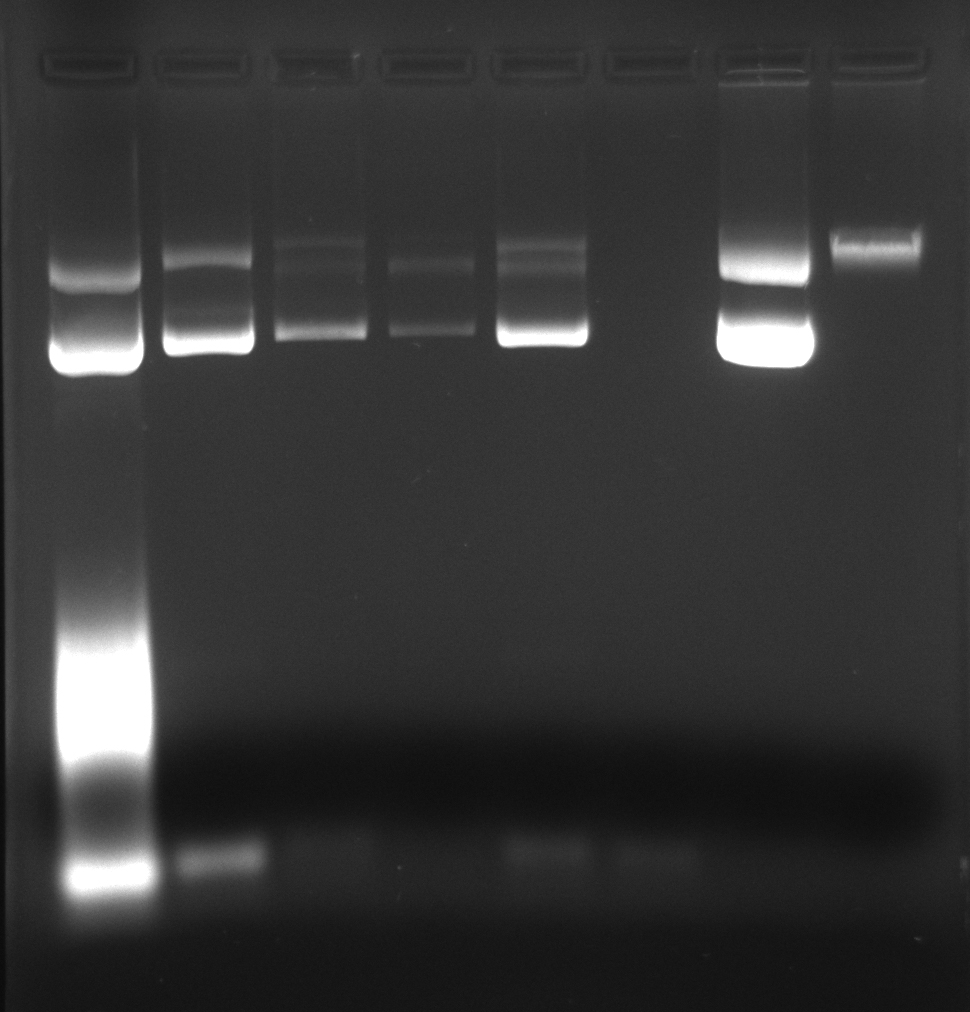
\includegraphics[width=5cm]{ima2}};
\begin{scope}[font=\scriptsize]
\node at (-2.025,2.8) {1};
\node at (-1.45,2.8) {2};
\node at (-0.85,2.8) {3};
\node at (-0.3,2.8) {4};
\node at (0.3,2.8) {5};
\node at (0.85,2.8) {6};
\node at (1.45,2.8) {7};
\node at (2.05,2.8) {8};
%
\draw (2.6,1.35) -- (2.75,1.35) -- (2.85,1.6) -- (3,1.6)  node[right] {gDNA};
\draw (2.6,1.25) -- (3,1.25) node[right] {pDNA (oc)};
\draw (2.6,0.9) -- (3,0.9) node[right] {pDNA (sc)};
\draw (2.6,-1) -- (3,-1) node[right] {RNA HMw};
\draw (2.6,-1.9) -- (3,-1.9) node[right] {RNA LMw};
\end{scope}
\end{tikzpicture}
\caption[Eletroforese horizontal em gel de agarose do processo MF-C/UF-C]{Análise por eletroforese horizontal em gel de agarose (1\%) do processo MF-C/UF-C: (1) lisado antes da adição de \cacldois\ 1\,M; (2) lisado após adição de \cacldois\ 1\,M; (3) permeado da microfiltração; (4) concentrado da microfiltração; (5) concentrado da ultrafiltração; (6) permeado da ultrafiltração; (7) amostra purificada de \pVAX\ pelo kit comercial da Qiagen; (8) Amostra de gDNA de \ecolidh, purificado com o kit da Promega.}
\label{fig:4dart3}
\end{figure}

\subsection{Ensaios de ultrafiltração}
\label{subsec:3p2art3}
\index{ultrafiltração}%
Após concluída a operação de diafiltração sólido/líquido, testou-se uma segunda operação de membranas para concentrar, e ao mesmo tempo, purificar o plasmídeo. Para isso, utilizou-se uma membrana de ultrafiltração com um ``cut-off'' de 100\,kDa, feita de um polímero fluorado, modelo \emph{FS40PP} da \emph{Alpha-Laval}, que tem um poro com um raio de 4.1\,nm \cite{meu1}.
\index{FS40PP}%
A concentração dos permeados provenientes dos testes MF-A, MF-B e MF-C foi efetuada à pressão constante de 1\,bar e a um fator de concentração volumétrico (VCF) de 3.0.
\index{fator!de concentração}%
Estes ensaios são denominados UF-A, UF-B e UF-C.
\index{UF-A|see{ultrafiltração}}%
\index{UF-B|see{ultrafiltração}}%
\index{UF-C|see{ultrafiltração}}%
\index{ultrafiltração!UF-A}%
\index{ultrafiltração!UF-B}%
\index{ultrafiltração!UF-C}%
Obtiveram-se fluxos consideravelmente mais altos nos ensaios UF-C quando comparados com os valores obtidos nos restantes dois ensaios, o que provavelmente se ficou a dever à remoção prévia dos contaminantes hidrofóbicos, tal como se pode verificar na figura~\ref{fig:5aart3}.
\index{contaminantes!hidrofóbicos}%
No entanto, os rendimentos de recuperação mais altos registaram-se nos ensaios UF-A (97$\pm$2\%) como indicado na figura~\ref{fig:5bart3}.
\index{rendimento!de recuperação}%
Nos ensaios UF-B e UF-C, os rendimentos obtidos foram (93$\pm$2\%) e (89$\pm$3\%), respetivamente, tal como se pode verificar na mesma figura. Uma vez que a concentração de pDNA medida nos permeados foi consistentemente muito reduzida para os testes UF-B e UF-C, observaram-se valores significativos de adsorção, $\sim$7 e $\sim$11\% respetivamente.
\index{adsorção!membrana}%
Nos ensaios UF-A verificou-se uma menor ocorrência de adsorção ($\sim$3\%). Observou-se permeação de contaminantes em todos os ensaios de ultrafiltração, o que levou a um significativo grau de purificação, dado que o plasmídeo foi sempre muito retido pela membrana.
\index{contaminantes!hidrofílicos}%
Para o caso dos contaminantes hidrofílicos, a sua remoção corresponde praticamente ao valor teórico considerando permeação total, que é igual a 66\% para um fator de concentração volumétrico de 3.0. Para os contaminantes hidrofóbicos verificou-se uma remoção de $20-40$\porcento, o que indica uma permeação observada de cerca de 0.5. 
\begin{figure}
	\centering
	\setlength\figureheight{6cm} 
	\setlength\figurewidth{6cm}
	% This file was created by matlab2tikz v0.3.3.
% Copyright (c) 2008--2013, Nico Schlömer <nico.schloemer@gmail.com>
% All rights reserved.
% 
% The latest updates can be retrieved from
%   http://www.mathworks.com/matlabcentral/fileexchange/22022-matlab2tikz
% where you can also make suggestions and rate matlab2tikz.
% 
% 
% 
\begin{tikzpicture}

\begin{axis}[%
width=\figurewidth,
height=\figureheight,
scale only axis,
xmin=1,
xmax=3.25,
xlabel={VDF},
ymin=0,
ymax=30,
ylabel={\fluxo\,[\micro\meter/s]},
legend style={at={(1.03,0.5)},anchor=west,draw=black,font=\scriptsize,fill=white,legend cell align=left}
]
\addplot [
color=black,
solid,
mark=*,
mark options={solid,fill=white,draw=black}
]
plot [error bars/.cd, y dir = both, y explicit,error bar style={solid}]
coordinates{
(1.108870968,23.26683292) +- (0.0,2.16957606)(1.245967742,20.57356608) +- (0.0,1.94513716)(1.431451613,18.17955112) +- (0.0,1.64588529)(1.665322581,16.3840399) +- (0.0,1.34663342)(2,14.96259352) +- (0.0,2.09476309)(2.5,13.69077307) +- (0.0,2.01995012)(2.943548387,13.24189526) +- (0.0,1.87032419)};
\addlegendentry{UF-A};

\addplot [
color=black,
dashed,
mark=*,
mark options={solid,fill=black,draw=black}
]
plot [error bars/.cd, y dir = both, y explicit,error bar style={solid}]
coordinates{
(1.112903226,22.81795511) +- (0.0,2.24438903)(1.25,15.11221945) +- (0.0,1.34663342)(1.427419355,11.97007481) +- (0.0,1.12219452)(1.665322581,10.32418953) +- (0.0,0.748129670000001)(2,9.351620948) +- (0.0,0.822942641999999)(2.5,8.753117207) +- (0.0,0.748129676)(3.008064516,8.453865337) +- (0.0,0.748129674999999)};
\addlegendentry{UF-B};

\addplot [
color=black,
dash pattern=on 1pt off 3pt on 3pt off 3pt,
mark=triangle*,
mark options={solid,fill=black,draw=black}
]
plot [error bars/.cd, y dir = both, y explicit,error bar style={solid}]
coordinates{
(1.112903226,24.83790524) +- (0.0,2.16957606)(1.25,23.04239401) +- (0.0,2.24438903)(1.427419355,21.17206983) +- (0.0,1.94513715)(1.665322581,19.52618454) +- (0.0,2.01995012)(2,17.80548628) +- (0.0,1.72069826)(2.504032258,16.3840399) +- (0.0,1.42144638)(3.004032258,15.86034913) +- (0.0,1.42144638)};
\addlegendentry{UF-C};

\end{axis}
\end{tikzpicture}%
	\caption[Fluxo de permeado em função do fator de concentração volumétrico (UF)]{Fluxo de permeado em função do fator de concentração volumétrico (VCF) para os ensaios de ultrafiltração. Condições operatórias: $p=1$\,bar, $\agitacao=760$\,\minmum, $T=25$\,\degreecelsius.}
	\label{fig:5aart3}
\end{figure}
\begin{figure}
\centering
\begin{tikzpicture}
\node[right,font=\scriptsize] at (0,5.75) {Ultrafiltração};
\begin{axis}[
	width=8cm,
	height=6cm,
	scale only axis,
	ybar,
	bar width=5pt,
	ymin=0,
	ymax=1.15,
	enlarge x limits=0.25,
	legend style={at={(0.5,-0.15),font=\scriptsize},
	anchor=north,legend columns=3,legend cell align=left},
	symbolic x coords={UF-A,UF-B,UF-C},
	xtick=data,
	]
\addplot[draw=black,fill=black,
	error bars/.cd,
	y dir=plus,y explicit]
coordinates {
	(UF-A,0.973568282) +- (UF-A,0.015418502)
	(UF-B,0.931718062) +- (UF-B,0.015418502)
	(UF-C,0.894273128) +- (UF-C,0.030837004)};
% Rend pVAX
\addplot[draw=black,fill=gray,
	error bars/.cd,
	y dir=plus,y explicit]
coordinates {
	(UF-A,0.665198238) +- (UF-A,0.030837004)
	(UF-B,0.599118943) +- (UF-B,0.039647577)
	(UF-C,0.698237886) +- (UF-C,0.094713656)};
% Rend Fil
\addplot[draw=black,fill=lightgray,
	error bars/.cd,
	y dir=plus,y explicit]
coordinates {
	(UF-A,0.292951542) +- (UF-A,0.099118943)
	(UF-B,0.213656388) +- (UF-B,0.044052863)
	(UF-C,0.691629956) +- (UF-C,0.052863436)};
% Rend Fob
%Ads pVAX
\addplot[error bars/.cd,
	y dir=plus,y explicit]
coordinates {
	(UF-A,0.022026432) +- (UF-A,0.028634361)
	(UF-B,0.059471366) +- (UF-B,0.024229075)
	(UF-C,0.101321586) +- (UF-C,0.028634361)};
%
\addplot[draw=black,pattern=north west lines,
	error bars/.cd,
	y dir=plus,y explicit]
coordinates {
	(UF-A,0.057268722) +- (UF-A,0.008810573)
	(UF-B,0.072687225) +- (UF-B,0.022026432)
	(UF-C,0.04845815) +- (UF-C,0.024229075)};
%
\addplot[draw=black,pattern=north east lines,
	error bars/.cd,
	y dir=plus,y explicit]
coordinates {
	(UF-A,0.066079295) +- (UF-A,0.011013216)
	(UF-B,0.160792952) +- (UF-B,0.079295154)
	(UF-C,0.303964758) +- (UF-C,0.085903084)};
\legend{Rendimento pDNA,Remoção c. hidrofílicos,Remoção c. hidrofóbicos,Adsorção pDNA,Adsorção c. hidrofílicos, Adsorção c. hidrofóbicos}
\end{axis}
\end{tikzpicture}
\caption[Valores de rendimento, adsorção e remoção (UF)]{Valores experimentais, obtidos nos testes de ultrafiltração, de adsorção e de rendimento de recuperação de pDNA e de adsorção e rendimentos de remoção de contaminantes hidrofílicos e de contaminantes hidrofóbicos.}
\label{fig:5bart3}
\end{figure}
\begin{figure}
\centering
\begin{tikzpicture}
\node at (0,0) {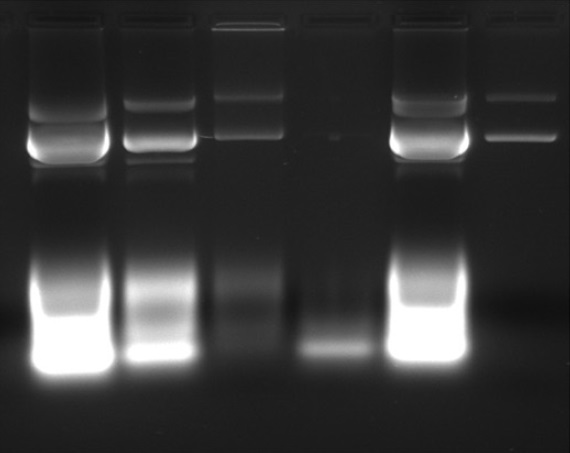
\includegraphics[width=5cm]{ima3}};
\begin{scope}[font=\scriptsize]
\node at (-1.95,2.2) {1};
\node at (-1.15,2.2) {2};
\node at (-0.3,2.2) {3};
\node at (0.45,2.2) {4};
\node at (1.3,2.2) {5};
\node at (2.1,2.2) {6};
\draw (2.6,1.15) -- (3,1.15) node[right] {pDNA (oc)};
\draw (2.6,0.8) -- (3,0.8) node[right] {pDNA (sc)};
\draw (2.6,-0.5) -- (3,-0.5) node[right] {RNA HMw};
\draw (2.6,-1.05) -- (3,-1.05) node[right] {RNA LMw};
\end{scope}
\end{tikzpicture}
\caption[Eletroforese horizontal em gel de agarose do processo MF-A/UF-A]{Análise por eletroforese horizontal em gel de agarose (1\porcento) do processo MF-A/UF-A: (1) Lisado; (2) permeado da microfiltração; (3) concentrado da microfiltração; (4) permeado da ultrafiltração; (5) concentrado da ultrafiltração; (6) amostra purificada de \pVAX.}
\label{fig:5cart3}
\end{figure}

Considerando os valores experimentais de fluxo de permeado, as permeações observadas teóricas para o pDNA, e para as várias espécies de RNA, podem ser estimadas ao longo dos diferentes processos de concentração para interpretar as diferenças entre o comportamento do plasmídeo e dos contaminantes (ver figura~\ref{fig:6art3}). Como se pode observar na figura~\ref{fig:6art3}(a), são esperados valores reduzidos de \permobs, ao longo do processo de ultrafiltração, um resultado que está de acordo com as reduzidas permeações observadas obtidas experimentalmente.
\index{ultrafiltração!permeação observada}%
Na mesma figura é ainda possível verificar que o modelo teórico prevê valores consideravelmente reduzidos de \permobs, quer para o RNA 23\,S quer para o RNA 16\,S. No entanto o mesmo não se verifica para o RNA 5\,S, o que provavelmente explica os valores intermédios de permeação observada de RNA total, como mencionado anteriormente.
\index{RNA!23\,S}%
\index{RNA!16\,S}%
\index{RNA!5\,S}%
Os resultados da análise por eletroforese, mostrados na figura~\ref{fig:5cart3}, confirmam esta ideia. Pode-se observar, na mesma figura, que ambas as isoformas do plasmídeo são retidas pela membrana.
\index{AGE}%
\index{isoforma}%
\begin{figure}
\centering
\begin{tikzpicture}

%FIGURA 6 DO ARTIGO 3

%\draw[help lines] (-4,-4) grid (14,21);
\begin{axis}[%Sobs vs FCv UF-A
	width=5cm,
	height=5cm,
	scale only axis,
	xmin=1,
	xmax=2.5,
	xlabel={VDF},
	ymin=-0.1,
	ymax=1.1,
	ylabel={\permobs},
	at={(0cm,14cm)},
	anchor=south west,
	]
\addplot[
color=black,
solid,
]
table[row sep=crcr]{
1.002184087 0.011655012\\
1.16599064 0.009324009\\
1.423712949 0.006993007\\
1.666146646 0.006993007\\
1.858346334 0.006993007\\
1.987207488 0.006993007\\
2.166302652 0.004662005\\
2.502652106 0.004662005\\
};

\addplot[
color=black,
dashed,
]
table[row sep=crcr]{
1.002184087 0.072261072\\
1.080811232 0.065268065\\
1.242433697 0.058275058\\
1.395319813 0.053613054\\
1.685803432 0.048951049\\
1.976287051 0.044289044\\
2.20124805 0.044289044\\
2.360686427 0.041958042\\
2.500468019 0.03962704\\
};

\addplot [
color=black,
dash pattern=on 1pt off 3pt on 3pt off 3pt,
%forget plot
]
table[row sep=crcr]{
1.002184087 0.146853147\\
1.085179407 0.132867133\\
1.264274571 0.114219114\\
1.458658346 0.102564103\\
1.585335413 0.095571096\\
1.76224649 0.090909091\\
1.939157566 0.086247086\\
2.122620905 0.083916084\\
2.312636505 0.081585082\\
2.500468019 0.079254079\\
};

\addplot [
color=black,
dotted,
%forget plot
]
table[row sep=crcr]{
1.002184087 0.913752914\\
1.133229329 0.883449883\\
1.375663027 0.836829837\\
1.613728549 0.808857809\\
1.808112324 0.79020979\\
2.089859594 0.773892774\\
2.282059282 0.769230769\\
2.502652106 0.764568765\\
};
\end{axis}

\begin{axis}[%Cm/Cb vs FCv UF-A
	width=5cm,
	height=5cm,
	scale only axis,
	xmin=1,
	xmax=2.5,
	xlabel={VDF},
	ymin=0,
	ymax=6,
	ylabel={\concm/\concb},
	at={(7cm,14cm)},
	anchor=south west,
	]
\addplot[
color=black,
solid,
]
table[row sep=crcr]{
1 4.868154158\\
1.06431853 4.430020284\\
1.19295559 3.711967546\\
1.405206738 3.018255578\\
1.540275651 2.738336714\\
1.767534456 2.409736308\\
1.941194487 2.227180527\\
2.166309342 2.093306288\\
2.393568147 1.983772819\\
2.500765697 1.935091278\\
};

\addplot[
color=black,
dashed,
]
table[row sep=crcr]{
1 2.288032454\\
1.098621746 2.068965517\\
1.169372129 1.947261663\\
1.379479326 1.716024341\\
1.617457887 1.569979716\\
1.821133231 1.472616633\\
1.99050536 1.436105477\\
2.11914242 1.39959432\\
2.273506891 1.37525355\\
2.417151608 1.350912779\\
2.502909648 1.338742394\\
};

\addplot [
color=black,
dash pattern=on 1pt off 3pt on 3pt off 3pt,
%forget plot
]
table[row sep=crcr]{
1 2.799188641\\
1.068606432 2.592292089\\
1.197243492 2.288032454\\
1.355895865 2.056795132\\
1.490964778 1.922920892\\
1.692496172 1.764705882\\
1.874732006 1.679513185\\
2.063399694 1.606490872\\
2.192036753 1.582150101\\
2.367840735 1.53346856\\
2.502909648 1.509127789\\
};

\addplot [
color=black,
dotted,
%forget plot
]
table[row sep=crcr]{
1 2.190669371\\
1.092189893 2.14198783\\
1.295865237 2.044624746\\
1.493108729 1.971602434\\
1.619601838 1.947261663\\
1.894027565 1.874239351\\
2.089127106 1.862068966\\
2.241347626 1.84989858\\
2.447166922 1.837728195\\
2.500765697 1.837728195\\
};
\end{axis}

\begin{axis}[%Sobs vs FCv UF-B
	width=5cm,
	height=5cm,
	scale only axis,
	xmin=1,
	xmax=2.5,
	xlabel={VDF},
	ymin=0,
	ymax=1.1,
	ylabel={\permobs},
	at={(0cm,7cm)},
	anchor=south west,
	]
\addplot[
color=black,
solid,
]
table[row sep=crcr]{
1 0.198135198\\
1.045865835 0.160839161\\
1.120124805 0.111888112\\
1.211856474 0.086247086\\
1.351638066 0.067599068\\
1.508892356 0.055944056\\
1.67925117 0.048951049\\
1.821216849 0.044289044\\
1.947893916 0.03962704\\
2.175039002 0.034965035\\
2.356318253 0.032634033\\
2.5 0.03030303\\
};

\addplot[
color=black,
dashed,
]
table[row sep=crcr]{
1 0.475524476\\
1.024024961 0.433566434\\
1.056786271 0.368298368\\
1.102652106 0.298368298\\
1.133229329 0.27039627\\
1.181279251 0.237762238\\
1.290483619 0.202797203\\
1.401872075 0.17948718\\
1.618096724 0.149184149\\
1.840873635 0.132867133\\
1.99375975 0.125874126\\
2.146645866 0.118881119\\
2.288611544 0.114219114\\
2.439313573 0.10955711\\
2.5 0.107226107\\
};

\addplot [
color=black,
dash pattern=on 1pt off 3pt on 3pt off 3pt,
%forget plot
]
table[row sep=crcr]{
1 0.804195804\\
1.028393136 0.724941725\\
1.085179407 0.582750583\\
1.150702028 0.48018648\\
1.224960998 0.417249417\\
1.299219969 0.377622378\\
1.473946958 0.317016317\\
1.655226209 0.284382284\\
1.899843994 0.256410256\\
2.100780031 0.242424242\\
2.277691108 0.233100233\\
2.408736349 0.226107226\\
2.5 0.221445221\\
};

\addplot [
color=black,
dotted,
%forget plot
]
table[row sep=crcr]{
1 0.955710956\\
1.063338534 0.8997669\\
1.133229329 0.850815851\\
1.220592824 0.813519814\\
1.336349454 0.778554779\\
1.528549142 0.750582751\\
1.64648986 0.738927739\\
1.853978159 0.722610723\\
2.081123245 0.715617716\\
2.32574103 0.710955711\\
2.5 0.708624709\\
};
\end{axis}

\begin{axis}[%Cm/Cb vs FCv UF-B
	width=5cm,
	height=5cm,
	scale only axis,
	xmin=1,
	xmax=2.5,
	xlabel={VDF},
	ymin=-5,
	ymax=70,
	ylabel={\concm/\concb},
	at={(7cm,7cm)},
	anchor=south west,
	]
\addplot[
color=black,
solid,
]
table[row sep=crcr]{
1 59.0070922\\
1.023913043 52.19858156\\
1.084782609 38.58156028\\
1.126086957 31.91489362\\
1.180434783 27.23404255\\
1.247826087 23.82978723\\
1.339130435 20.56737589\\
1.484782609 17.0212766\\
1.660869565 14.32624113\\
1.823913043 12.76595745\\
2.013043478 11.34751773\\
2.256521739 10.21276596\\
2.5 9.219858156\\
};

\addplot[
color=black,
dashed,
]
table[row sep=crcr]{
1 15.03546099\\
1.030434783 13.04964539\\
1.07826087 10.4964539\\
1.152173913 8.085106383\\
1.236956522 6.95035461\\
1.317391304 6.241134752\\
1.469565217 5.24822695\\
1.606521739 4.822695035\\
1.752173913 4.397163121\\
1.913043478 4.113475177\\
2.058695652 3.829787234\\
2.204347826 3.687943262\\
2.284782609 3.687943262\\
2.434782609 3.404255319\\
2.5 3.404255319\\
};

\addplot [
color=black,
dash pattern=on 1pt off 3pt on 3pt off 3pt,
%forget plot
]
table[row sep=crcr]{
1 15.31914894\\
1.065217391 11.91489362\\
1.130434783 9.503546099\\
1.197826087 8.226950355\\
1.32173913 6.95035461\\
1.458695652 6.09929078\\
1.639130435 5.390070922\\
1.815217391 4.964539007\\
2.054347826 4.680851064\\
2.263043478 4.397163121\\
2.5 4.255319149\\
};

\addplot [
color=black,
dotted,
%forget plot
]
table[row sep=crcr]{
1 2.269503546\\
1.091304348 2.127659574\\
1.302173913 1.843971631\\
1.608695652 1.70212766\\
1.930434783 1.560283688\\
2.12826087 1.70212766\\
2.367391304 1.560283688\\
2.5 1.560283688\\
};
\end{axis}

\begin{axis}[%Sobs vs FCv UF-C
	width=5cm,
	height=5cm,
	scale only axis,
	xmin=1,
	xmax=2.5,
	xlabel={VDF},
	ymin=0,
	ymax=1.1,
	ylabel={\permobs},
	at={(0cm,0cm)},
	anchor=south west,
	legend style={at={(6cm,-1.5cm)},legend columns=2,anchor=center,font=\scriptsize,draw=black,fill=white,legend cell align=left}
	]
\addplot[
color=black,
solid,
]
table[row sep=crcr]{
1.002184087 0.948837209\\
1.065522621 0.918604651\\
1.334165367 0.802325581\\
1.476131045 0.73255814\\
1.631201248 0.662790698\\
1.821216849 0.597674419\\
1.958814353 0.565116279\\
2.135725429 0.534883721\\
2.336661466 0.509302326\\
2.500468019 0.490697674\\
};
\addlegendentry{\pVAX};

\addplot[
color=black,
dashed,
]
table[row sep=crcr]{
1.002184087 0.979069767\\
1.096099844 0.979069767\\
1.24024961 0.979069767\\
1.386583463 0.979069767\\
1.543837754 0.979069767\\
1.685803432 0.979069767\\
1.987207488 0.979069767\\
2.20124805 0.979069767\\
2.417472699 0.979069767\\
2.5 0.979069767\\
};
\addlegendentry{RNA 23\,S};

\addplot [
color=black,
dash pattern=on 1pt off 3pt on 3pt off 3pt,
%forget plot
]
table[row sep=crcr]{
1.002184087 0.997674419\\
1.159438378 0.993023256\\
1.445553822 0.98372093\\
1.642121685 0.972093023\\
1.816848674 0.960465116\\
2.013416537 0.951162791\\
2.194695788 0.946511628\\
2.428393136 0.941860465\\
2.5 0.941860465\\
};
\addlegendentry{RNA 16\,S};

\addplot [
color=black,
dotted,
%forget plot
]
table[row sep=crcr]{
1.002184087 0.962790698\\
1.172542902 0.946511628\\
1.535101404 0.91627907\\
1.770982839 0.9\\
1.934789392 0.890697674\\
2.120436817 0.88372093\\
2.292979719 0.881395349\\
2.5 0.879069767\\
};
\addlegendentry{RNA 5\,S};
\end{axis}

\begin{axis}[%Cm/Cb vs FCv UF-C
	width=5cm,
	height=5cm,
	scale only axis,
	xmin=1,
	xmax=2.5,
	xlabel={VDF},
	ymin=-10,
	ymax=200,
	ylabel={\concm/\concb},
	at={(7cm,0cm)},
	anchor=south west,
	]
\addplot[
color=black,
solid,
]
table[row sep=crcr]{
1 179.5955056\\
1.112087912 170.2921348\\
1.279120879 156.5393258\\
1.487912088 137.9325843\\
1.668131868 122.5617978\\
1.824175824 112.8539326\\
1.98021978 105.9775281\\
2.107692308 101.9325843\\
2.287912088 97.48314607\\
2.432967033 94.24719101\\
2.5 93.03370787\\
};

\addplot[
color=black,
dashed,
]
table[row sep=crcr]{
1 31.14606742\\
1.171428571 31.14606742\\
1.397802198 31.14606742\\
1.681318681 31.14606742\\
1.905494505 31.14606742\\
2.118681319 31.14606742\\
2.342857143 31.14606742\\
2.5 31.14606742\\
};

\addplot [
color=black,
dash pattern=on 1pt off 3pt on 3pt off 3pt,
%forget plot
]
table[row sep=crcr]{
1 19.01123596\\
1.206593407 18.60674157\\
1.514285714 18.20224719\\
1.810989011 18.20224719\\
2.059340659 17.79775281\\
2.301098901 17.79775281\\
2.5 17.79775281\\
};

\addplot [
color=black,
dotted,
%forget plot
]
table[row sep=crcr]{
1 2.426966292\\
1.217582418 2.02247191\\
1.615384615 2.02247191\\
1.892307692 2.02247191\\
2.206593407 2.02247191\\
2.406593407 2.02247191\\
2.5 2.02247191\\
};
\end{axis}

\begin{scope}[font=\large]
\node[right] at (0,19.5) {a)};
\node[right] at (7,19.5) {b)};
\node[right] at (0,12.5) {c)};
\node[right] at (7,12.5) {d)};
\node[right] at (0,5.5) {e)};
\node[right] at (7,5.5) {f)};
\end{scope}

\begin{scope}[font=\scriptsize]
\node[right] at (0,18.75) {UF-A};
\node[right] at (7,18.75) {UF-A};
\node[right] at (0,11.75) {UF-B};
\node[right] at (7,11.75) {UF-B};
\node[right] at (0,4.75) {UF-C};
\node[right] at (7,4.75) {UF-C};
\end{scope}

\end{tikzpicture}
\caption[Permeação e polarização de concentração previstas em função do fluxo]{Permeação observada e polarização de concentração previstas em função do fluxo, para as espécies indicadas, ao longo dos ensaios de ultrafiltração (UF-A, UF-B e UF-C). Utilizaram-se os modelos CSC e FJC, considerando efeitos de carga, para $\raioporo=4.1$\,nm. Condições: \fluxo\ como indicado na figura~\ref{fig:5aart3}, $\agitacao=760$\,\minmum, $T=25$\,\degreecelsius.}
\label{fig:6art3}
\end{figure}

A polarização de concentração não foi excessiva durante os ensaios UF-A, como se pode observar a partir das simulações representadas na figura~\ref{fig:6art3}(b), o que provavelmente explica a menor adsorção do plasmídeo verificada nestes ensaios.
\index{polarização de concentração}%
Para os outros ensaios, o modelo prevê um aumento da polarização de concentração, devido ao aumento da força iónica, tal como se pode verificar nas figuras~\ref{fig:6art3}(d)~e~(f).
\index{força iónica}%
Uma elevada polarização de concentração pode levar ou a uma maior permeação do plasmídeo (e RNA) ou a uma maior adsorção nos ensaios UF-B e UF-C, quando comparados com os ensaios UF-A. Tal como se pode concluir pela análise dos resultados experimentais, mostrados na figura~\ref{fig:5bart3}, o aumento de polarização de concentração conduziu essencialmente a um aumento do valor da adsorção. Assim, as permeações observadas previstas, indicadas na figura~\ref{fig:6art3}(c)~e~(e), não são corretas devido à ocorrência de adsorção. A elevada tendência do pDNA para se adsorver em membranas, em condições de elevada polarização de concentração, foi previamente identificada no capítulo~\ref{chap:art2}. Foi observada uma elevada permeação de proteínas através da membrana de ultrafiltração, com exceção dos ensaios com o tampão ``B'', tal como se pode observar na tabela~\ref{tab:3art3}. Pela análise de lisados por SEC, discutida no capítulo~\ref{cha:pra}, pode-se concluir que o material proteico presente nos lisados tem uma menor massa molecular que o LMw\,RNA, o que indica que deve permear pela membrana. No caso dos ensaios com o tampão ``B'', a permeação de proteínas deverá ter sido influenciada pelo maior grau de colmatação da membrana, tal como se pode observar na figura~\ref{fig:5aart3}.
\begin{table}%
\caption[Proteína total e DNA genómico (gDNA) nos concentrados (UF)]{Proteína total e DNA genómico (gDNA) nos concentrados dos ensaios de ultrafiltração e os seus rendimentos de remoção (\remocaodois) na operação de ultrafiltração}
\label{tab:3art3}
\centering
\begin{tabular*}{12cm}{lr@{}l @{\extracolsep{\fill}} lll}
\toprule
Tampão &\multicolumn{2}{l}{Proteínas [\micro g/mL]} &  \remocaodois\ (\porcento) & gDNA [\micro g/mL] & \remocaodois (\porcento) \\
\midrule
``A'' & 64 & & 65 & 92 & 28 \\
``B'' & 166 & & 22 & 44 & 20 \\
``C'' & 55 & & 59 & 17 & -5 \\
\bottomrule
\end{tabular*}
\end{table}

Observou-se uma permeação significativa de gDNA para os tampões ``A'' e ``B'', o que indica a presença de fragmentos de gDNA de menores dimensões que o plasmídeo, que por sua vez é retido.
\index{tampão!MF-A}%
\index{tampão!MF-B}%
A maior remoção de gDNA foi verificada nos ensaios UF-A, seguidos dos ensaios UF-B e por fim dos ensaios UF-C, onde não se observou remoção de gDNA. Assim, quando a re-dissolução de gDNA é alta no passo de microfiltração a remoção é igualmente alta no passo de ultrafiltração (ver tabelas~\ref{tab:2art3}~e~\ref{tab:3art3}), o que sugere que a re-dissolução do gDNA é provocada pela quebra das cadeias.
\index{DNA genómico!redissolução}%
A partir dos dados de remoção de gDNA obtidos nos ensaios UF-A e UF-B (indicados na tabela~\ref{tab:3art3}) a massa molecular média dos fragmentos de gDNA que chegam à operação de ultrafiltração pode ser estimada como descrito em \cite{meu3}.
\index{DNA genómico!fragmentos}%
Considerando que estes fragmentos são compostos por DNA linear de dupla cadeia (dsDNA) o número de pares de bases deverá ser, de acordo com os cálculos efetuados em \cite{meu3}, 205 no caso do tampão ``A'' e 1700 no caso do tampão ``B''. Estes valores correspondem a raios hidrodinâmicos de 16\,nm e 59\,nm, respetivamente, o que indica que estes fragmentos são consideravelmente menores que o plasmídeo usado, cujo raio hidrodinâmico é de 83\,nm. Pode-se assim concluir que apesar do gDNA se re-dissolver no passo de microfiltração, os fragmentos resultantes podem ser removidos no passo de ultrafiltração. O grau de remoção pode ser assim melhorado com recurso a uma diafiltração neste segundo passo, uma vez que o plasmídeo é retido pela membrana. No entanto, e em especial para o caso do RNA de alto peso molecular (HMw\,RNA), não é esperado que se venham a obter rendimentos de remoção muito elevados, dado os reduzidos valores verificados da permeação desta biomolécula. No capítulo~\ref{chap:art4} a separação pDNA/RNA é estudada em melhor detalhe.

\section{Conclusões}
Os modelos teóricos desenvolvidos de transferência de massa para cadeias CSC e FJC, usados para prever a permeação de pDNA e RNA na microfiltração de lisados, e subsequente concentração, foram aplicados com sucesso, uma vez que os resultados obtidos nos dois passos de membranas podem ser explicados com base neste desenvolvimento teórico.

A recuperação de um plasmídeo com 6050\,bp, a partir de lisados, foi efetuada de forma eficiente por uma operação de microfiltração, usando uma membrana hidrofílica de Nylon, com um tamanho de poro nominal de 0.2\,\micro m. Este tamanho de poro, bem como as condições operacionais, foi selecionado com base nas previsões teóricas para que se evite, quer uma excessiva polarização de concentração do plasmídeo, quer a adsorção do mesmo na superfície da membrana. Verificou-se que outros contaminantes, nomeadamente RNA, proteínas e gDNA, permeiam através da membrana de microfiltração juntamente com o plasmídeo. A adição de \cacldois\ 1\,M aos lisados conduziu à remoção quase completa do RNA, tal como esperado pelos resultados encontrados na literatura. Verificou-se igualmente que a adição deste sal reduziu significativamente o conteúdo de gDNA nos lisados, gDNA esse que tende a se re-dissolver durante a operação de microfiltração, o que se observou em todos os ensaios. Um aumento da força iónica da solução de diafiltração pode reduzir esta tendência, no entanto não a elimina por completo.

Estudou-se uma operação de ultrafiltração para purificar e concentrar o plasmídeo após a microfiltração. Apesar do RNA de alto peso molecular ser completamente retido pela membrana, observou-se alguma permeação de RNA de baixo peso molecular, tal como previsto pelo modelo. Proteínas e gDNA podem ser consideravelmente removidos por ultrafiltração. A elevada permeabilidade dos fragmentos de gDNA na operação de ultrafiltração pode ser explicada pelos seus reduzidos tamanhos, que se estimou serem consideravelmente inferiores ao plasmídeo usado. Assim, apesar de se verificar uma significativa re-dissolução de gDNA no passo de microfiltração, os fragmentos presentes em solução são de tamanho reduzido e podem ser separados do plasmídeo num passo de ultrafiltração.
